\chapter{数と演算}\label{chapt:num_calc}

%{\small 君は「はじめに」を全部, 隅々まで読みましたか? 
%読まずに進むと, 誤った方法で勉強することになり, 時間と努力を無駄にします。}\\


%\section{数学の体系の再構築}

君はこれまでたくさん算数・数学を勉強してきたので, 
数の掛け算や割り算などは朝飯前だろう。でもそれは「やり方を知ってる」
だけで, 「そうなる理由」は知らないのでは? 例えば, 
\begin{itemize}
\item 1たす1はなぜ2なの?
\item マイナスとマイナスをかけるとなぜプラス?
\end{itemize}
などに, 自信を持って答えられるだろうか?

大学では, そういう「基礎」にこだわって, 数学の体系を再構築すること
から始める。そうしないと, より高度で強力な数学を築くことができないのだ。\\


\section{等号}\label{sec:equality}

"="という記号を等号という。数学に等号はつきものだ。まず等号の意味をはっきりさせよう。

2つのものごと$a, b$が互いに等しいとき, 
\begin{eqnarray}a=b\end{eqnarray}
と書く。そして, 以下の3つ全てが常に成り立つということを, 認めよう:
\begin{eqnarray}
&&\text{$a$が何であっても, $a=a$である。}\label{eq:equality01}\\
&&\text{$a=b$のとき, $b=a$である。}\label{eq:equality02}\\
&&\text{$a=b$かつ$b=c$のとき, $a=c$である。}\label{eq:equality03}
\end{eqnarray}
ちょっと待った! 君は今, このへんを読んで, 「当たり前の話でダルいな」
と感じて読み飛ばそうとしたのでは? そういうのは大学では災いの元。
\eref{eq:equality01}$\sim$\eref{eq:equality03}は
等号の\underline{公理}\index{こうり@公理}だ。公理とは, 
学問における論理の前提であり, 出発点であり, 「それらは無条件に
成り立つ」と合意するもの。言い換えれば, これらは
等号の定義, つまり「等しいという関係」の\underline{定義}だ。
話の順序を正せば, 『「等しいという関係」は
\eref{eq:equality01}$\sim$\eref{eq:equality03}を満たす』
のではなく, 
『\eref{eq:equality01}$\sim$\eref{eq:equality03}
を満たす関係を, 数学では「等しい」という』のだ。\mv

これをよくわかっておらず, \textgt{意味の違う量どうしを
なんとなく等号で結んでしまう悪癖}\label{badhabit_equality}
をもつ人は多い。

\begin{q}\label{q:badhabit_equality}
\begin{eqnarray}
\text{A君は学生である。}
\end{eqnarray}
ということを, 
\begin{eqnarray}
\text{A君 $=$学生}\label{eq:badhabit_equality2}
\end{eqnarray}
と書いてしまう人がいる。すると, \eref{eq:equality02}より, 
\begin{eqnarray}
\text{学生 $=$ A君}\label{eq:badhabit_equality4}
\end{eqnarray}
となってしまう。何か変。さらに, もしB君も学生であれば, 
\begin{eqnarray}
\text{B君 $=$学生}\label{eq:badhabit_equality6}\\
\text{学生 $=$B君}\label{eq:badhabit_equality7}
\end{eqnarray}
となり, \eref{eq:equality03}を\eref{eq:badhabit_equality2}と
\eref{eq:badhabit_equality7}に適用すれば, 
\begin{eqnarray}
\text{A君 $=$ B君}\label{eq:badhabit_equality8}
\end{eqnarray}
となって, A君とB君は同一人物になってしまう! この話は, 
どこでどのように間違えたか?\end{q}


\section{足し算・掛け算と自然数}

次に, 「数とは何か?」を考えよう。

まず, 「この世に1という数が存在する」ということを, 無条件に受け入れよう。
でなければ数学は始まらぬ。そして, 「1を繰り返し足すことによって, 
新たな数を作ることができる」と約束しよう。そうやってできる数を
\underline{自然数}\index{しぜんすう@自然数} (natural number)
と呼ぶ(定義)。それが, $1,\, 2,\, 3,\, \cdots$などの数だ。
\begin{exmpl}
2とは, $1+1$のことである(定義)。$1+1=2$という式は, 
計算の結果ではなく, 2という数の定義。(例おわり)\end{exmpl}\mv

以後, 「左辺を右辺によって定義する」ような等式には, 普通の等号"="ではなく, ":="という等号
を使おう(:はコロンという記号)。つまり, :=という記号が出てきたら, 左辺は右辺
によって初めて意味づけられるのだ, と解釈すればOK。上の例で言えば, 
\begin{eqnarray}
2:=1+1
\end{eqnarray}
だ(決して$1+1:=2$ではない)。\mv

0は自然数でない。なぜ? 自然数は「1を繰り返し足してできる数」
と定義されたが, 1を何回足しても0にはならないから。\mv

次に, 自然数どうしの足し算というものを考える。例えば2+3は,
\begin{eqnarray*}
2+3=(1+1)+(1+1+1)=1+1+1+1+1
\end{eqnarray*}
というふうに, 「1を繰り返し足すこと」に立ち返って定義しよう。\mv

次に, 自然数どうしの掛け算というものを考える。例えば2を3回足すことを, 
「2に3を掛ける」と呼び, $2\times3$と書く。一般に, $a, b$を
任意の自然数として, 「$a$に$b$を掛ける」とは「$a$を$b$回足すこと」
と定義しよう。\mv

これで, 自然数と, その足し算と掛け算が定義できた。どれも小学1, 2年生
で習ったことなのに, その理屈はなかなか深いではないか!\\


\section{引き算と整数}

次に引き算を定義しよう。数$a, b$について, 
\begin{eqnarray}
a=b+x\text{を満たすような数$x$を求めること}\label{eq:def_subtract}
\end{eqnarray}
を「$a$から$b$を引く」と呼び, $a-b$と書く。

自然数から自然数を引くと, 自然数になることもならないこともある。例えば
$5-2$は自然数(3)だが, $2-5$は自然数ではない。
そこで, 自然数から自然数を引いてできる数(それは必ずしも自然数ではない)
を考えよう。そのような数を\underline{整数}\index{せいすう@整数} (integer)と呼ぶ(定義)。

例えば2は自然数だが, 3という自然数から1という自然数を引いてもできるので, 整数でもある。
同様に考えれば, どんな自然数も整数だ。つまり, 自然数は整数でもある。
一方, $2-2=0$だから, 0は整数である。$1-2$, $1-3$などを考えれば, $-1, -2, \cdots$
なども整数。すなわち, 整数は, \\
  $\cdots$, $-3$, $-2$, $-1$, 0, 1, 2, 3, $\cdots$\\などの数である。

\section{割り算と有理数}

次に割り算を定義しよう。数$a, b$について, 
\begin{eqnarray}
a=b\times x\text{を満たすような数$x$を求めること}\label{eq:def_mult}
\end{eqnarray}
を「$a$を$b$で割る」と呼び, $a\div b$とか$\frac{a}{b}$とか$a/b$
と書く。ただし, 「0で割る」ことはできないと約束する。

整数を整数(0以外)で割ると, 整数になることもあれば, ならないこともある。
例えば$6\div 3$は整数(2)だが, $5\div4$は整数にはならない。
そこで, 整数を整数(0以外)で割ってできる数を考えよう。すなわち, 
2つの整数$n, m$ (ただし$m\ne0$とする)によって, 
\begin{eqnarray}
\frac{n}{m}
\end{eqnarray}
と表される数を考える。そのような数を
\underline{有理数}\index{ゆうりすう@有理数} (rational numberまたはquotient number)
と呼ぶ(定義)。ここで, 任意の整数$n$は, $n/1$と表すことができるので有理数でもある。
つまり, 整数は有理数でもある。

\begin{q}\label{q:alg_num0}
 自然数・整数・有理数を, それぞれ定義せよ。
\end{q}
\mv

\section{実数}

ところで, 円の周長を直径で割って得られる数を\underline{円周率}\index{えんしゅうりつ@円周率}
という(定義)。円周率は$\pi$という記号で表す。$\pi$は, $3.141592\cdots$
という無限に続く小数になるが, これはどんな整数$n, m$をもってしても, $n/m$というふう
には表現できない
\footnote{その証明は難しいのでここには載せない。興味があれば「円周率 無理数 証明」
で検索してみよう。でも君の今の数学力では理解できないだろうけどね。}。
同様に, $\sqrt{2}$, つまり「2乗したら2になるような正の数」は, $1.41421356\cdots$
という無限に続く小数になるが, これも, どんな整数$n, m$をもってしても, 
$n/m$というふうには表現できない\footnote{その証明は難しくはないが, 
「背理法」という考え方が必要なので, ここには載せない。}。
従って, $\pi$や$\sqrt{2}$は有理数ではない。このように, 無限に続く
小数で表現され, なおかつ有理数でないような数のことを
\underline{無理数}\index{むりすう@無理数} (irrational number)という。
有理数と無理数をあわせて, \underline{実数}\index{じっすう@実数} (real number)と呼ぶ
\footnote{実は, この定義は不完全である。無理数や実数の完全な
定義は, かなり難しい。数学類や数学科に進んだ学生は, ここで苦しむ
のだが, 我々は生物資源学類だから, ここはスルーして先に進もう。
「いや, 気になる!」という人は, 「実数の定義」で検索してみよう!}。\\


\section{定義について}\index{ていぎ@定義}

ここまでわずか数ページの中に「定義」という言葉が何回も出てきた! 
でも, 君は「定義」ってどういうことか, わかっているだろうか?

定義とは, 言葉の意味を規定すること。Aという言葉の定義は, 
「AとはBである」とか, 「BであるようなものをAと呼ぶ」という形式の文章
になる。ただしそこには暗黙のルールがある。\mv

まず, 定義は, 既に定義されている言葉だけで記述しなければダメ。例えば, 
「自然数とは, 1以上の整数である」はダメだ。なぜなら, 整数は自然数が
定義された後に, 自然数を使って定義されるものであり, 自然数の定義の
時点では, 整数はまだ定義されていないからだ。\mv

次に, 定義は, その言葉の指し示す対象を, 過不足無く特定できなければダメ。
例えば, 「自然数とは, 1, 2, 3等のことである」というのは, 4以上の
自然数についてきちんと述べていないからダメ。また例えば, 「自然数とは, 
ある種の整数である」は, $-1$や$-3$が自然数なのかどうかわからないからダメ。\mv

また, 定義は, 必要最低限のことだけが入っていなければダメ。
蛇足があってはダメだ。例えば, 
「$\sqrt{2}$とは, 2乗したら2になるような正の無理数」というのはダメ。
「無理数」が蛇足だ。「2乗したら2になるような正の数」という条件だけで
「2の平方根」は決まる。それをもとに, $\sqrt{2}$が無理数である
ことが証明されるのだ。

ちなみに, 定義から論理的に導かれる事柄を, 定理\index{ていり@定理}という。
「$\sqrt{2}$は無理数」というのは, 定義ではなく定理。\mv

\begin{q}\label{q:alg_def_pi} 円周率とは? という問に, A君は「3.14」と
答えた。それを聞いたB君は, 「それは違う。3.1415926, 以下, ずっと値が続く数だよ」
と言った。B君の発言はA君の答より少しはましだが, 正解とは言えない。なぜか?
\end{q}

\begin{faq}{\small\textgt{高校ではそんなに定義定義と言われ
なかったし, 他学類でも\underline{定義を覚えろ}なんて言われていないようですが}
 ... そのかわり高校では頻繁にテストがあったし, 他学類では週に
何回も数学の授業があります。それだけやってれば, 大事な定義は自然
に覚えちゃう。でも資源は忙しいのです。週1回しか数学の授業がない
ので, 覚えるべき定義をさっさと覚えることが必要です。考えるだけでは
理解しにくいことも, 覚えちゃえば, その後でじわじわと理解できるのです。
もし資源が「数学は暗記科目じゃない!」みたいな美しいスローガンで
のんびりやったら, 多分, 1年間で高校数学の復習すら終わらないよ。}\end{faq}

\begin{faq}{\small\textgt{先生は, これらの定義をどうやって覚えたのですか?} 
... 意識して覚えたのでなく, たくさん時間をかけて数学の体系を
自分なりに構築し, 一つ一つの概念について, ベストな定義を考えて
いきました。ところがそれは, どの本にも書かれている定義とほとんど
同じだったのです。時間の無駄でした。若くて愚かでした。数学では, 
個々の定義は徹底的に考え尽くされているのです。}\end{faq}

\begin{faq}{\small\textgt{定義と公理の違いがわかりません} 
... ほぼ同じです。強いて言えば, 公理の方が大げさな感じです。}\end{faq}
\mv

さて, 驚くべきことに, ひとつの事柄の定義は, ひとつとは限らず, 
場合によっては, 複数ありえるのだ。例えば円周率$\pi$は, 「円周の長さを
その円の直径で割ったもの」と定義するのが普通だが, 
\begin{eqnarray*}
\pi=4\times\Bigl(\frac{1}{1}-\frac{1}{3}+\frac{1}{5}-\frac{1}{7}+\cdots\Bigr)
\end{eqnarray*}
というふうに, 「奇数の逆数に, 正負交互に符号をつけて無限に足し合わせ, 最後に4倍したもの」
とも定義できるのだ! これはだいぶ先の大学の数学でないと理解
できないから, 今はわからなくてもOK(気になる人は\pref{q:univ_Taylor5}参照)。これを
$\pi$と定義すれば, それが「円周の長さをその円の直径で割ったもの」
に等しいということが数学的に証明でき, そのことは定理となるのだ。\mv

\begin{faq}{\small\textgt{定義が複数あるのなら, どれを
覚えればいいのですか? ていうか, 複数あるなら, 覚える意味, 無くないですか?} 
... ごもっとも。でも, まず代表的な定義を覚えましょう。でないと始まらない。
そのうち, 他の定義もあり得るということがわかってきます。}\end{faq}
\mv

ところで, 君が科学的な文章(レポートや答案など)を書くときは, 「記号の定義」が
重要である。例えば, 「円の面積の公式は?」と聞かれて「$\pi r^2$です」と答える
のは, 不十分。$\pi$が円周率を表すことは数学のルールとしてOKだが, $r$という
記号が何かは, 数学の中ではルールとして決まってはいないので, 「半径を$r$とする」
という宣言, つまり, $r$という記号の定義を述べねばダメなのだ。大事なことなので
大きく書いておこう:
\begin{itembox}{約束}
数学のルールとして定まった記号以外の記号は, 必ず定義してから使うこと。
\end{itembox}

どのような記号が数学のルールで定まっているのか? とりあえず, 
0, 1, 2, 3, $\cdots$という数字や, $=$, $+$, $-$, $\times$, $\div$, 
$\int$, $\sum$などの演算記号, $\pi$, $e$などの特別な定数, 
$\cos$, $\sin$などの関数記号, 等々。他にも, 第\ref{chapt_logic}章
に書いてある記号が, それにあたる。\\



\section{無限大}

さて, 先ほど, 「何かを0で割ることはできない」と述べたが, 0に近い数で
割ることはできる。例えば, 1を0.0001で割ると, 
$1/0.0001=10000$になる。あるいは, 1を$-0.0001$で割ると, $-10000$になる。
このように, 0に近い数で, 0でない何かを割ると, その結果は非常に大きな数になったり
非常に小さな数(マイナスの大きな数)になる。「割る数」を0に近づければ近づける
ほど, その傾向は際限なく激しくなる。際限なく大きくなる様子を, 象徴的に
\underline{無限大}\index{むげんだい@無限大} (infinity)と呼び, $\infty$という記号で表す。
あるいは際限なく小さな数(マイナスの大きな数)になる様子を, 「負の無限大」
と呼び, $-\infty$という記号で表す。

そういうふうに考えれば, 
\begin{eqnarray}
&&1\div 0 = \infty\text{ または, }\nonumber\\
&&1\div 0 = -\infty
\end{eqnarray}
と言えなくもなさそうだが, \textgt{これはダメ}。というのも, 
$\infty$は, 「数」ではないのだ。
あくまで「0での割り算はできない」という立場を貫こう。\mv

\begin{faq}{\small\textgt{「示せ」と「証明せよ」は同じことですか?}
... 同じです。}\end{faq}

\begin{faq}{\small\textgt{証明せよ, と言われても, 何を既知としてよいかわかりません}
... 定義と公理, そして, 自分がすでに(既出の問題などで)証明したこと(定理)は, 既知として構いません。}\end{faq}

\begin{faq}{\small\textgt{「証明の終わり」の印に指定はありますか?}
... 慣習的には, Q.E.D.とか, 「証明終」とか, 2本斜線とか, ■が使われます。}\end{faq}



\section{四則演算}\label{sec:realnum_calc}

足し算は「加算」\index{かさん@加算}, 
引き算は「減算」\index{げんさん@減算}, 
掛け算は「乗算」, \index{じょうさん@乗算} 
割り算は「除算」\index{じょさん@除算}とも呼ぶ。
加算・減算・乗算・除算の4つをまとめて\underline{四則演算}\index{しそくえんざん@四則演算}
とか\underline{加減乗除}\index{かげんじょうじょ@加減乗除}と呼ぶ。
加算・減算・乗算・除算の結果のことを, それぞれ和・差・積・商と呼ぶ。\\

任意の実数$a, b, c$について, 以下のようなルールが成り立つのは, 中学校
までの経験から自明だろう。
\begin{eqnarray}
&&a+b=b+a\label{eq:axiom_num_sum_exch}\\
&&(a+b)+c=a+(b+c)\label{eq:axiom_num_sum_assoc}\\
&&a+0=a\label{eq:axiom_num_zero}\\
&&a\text{に足して0になる数, つまり}\nonumber\\
&&\quad a+(-a)=0\quad\text{となる数「$-a$」がある。}\label{eq:axiom_num_sum_inv}\\
&&a\times b=b\times a\label{eq:axiom_num_mult_exch}\\
&&(a\times b)\times c=a\times(b\times c)\label{eq:axiom_num_mult_assoc}\\
&&a\times1=a\label{eq:axiom_num_one}\\
&&a\ne0\text{ならば, $a$に掛けて1になる数, つまり}\nonumber\\
&&\quad a\times(1/a)=1\quad\text{となる数「$1/a$」がある。}\label{eq:axiom_num_mult_inv}\\
&&a\times(b+c)=a\times b+a\times c\label{eq:axiom_num_distr}\\
&&0\neq1\label{eq:axiom_num_0neq1}
\end{eqnarray}

\eref{eq:axiom_num_sum_exch}, \eref{eq:axiom_num_mult_exch}のように, 
計算の順序を逆にしても結果が変わらない, という性質のことを, \underline{交換法則}
\index{こうかんほうそく@交換法則}という。\eref{eq:axiom_num_sum_exch}は
和の交換法則が成り立つことを, \eref{eq:axiom_num_mult_exch}は
積の交換法則が成り立つことを言っている。

\eref{eq:axiom_num_sum_assoc}, \eref{eq:axiom_num_mult_assoc}の
ように, 同種の計算が複数ある場合にどこから手をつけても結果が変わらない, 
という性質のことを, \underline{結合法則}\index{けつごうほうそく@結合法則}という。
\eref{eq:axiom_num_sum_assoc}は和の結合法則, 
\eref{eq:axiom_num_mult_assoc}は積の結合法則が, それぞれ成り立つ
ことを言っている。

\eref{eq:axiom_num_distr}は, \underline{分配法則}\index{ぶんぱいほうそく@分配法則}と呼ばれる。\\

ところで, 振り返ってみると, そもそも掛け算は「自然数を自然数回, 足すこと」
と定義した。つまり, 自然数$a, b$について, 「$a$を$b$回足すこと」を$a\times b$
と定義した。\textgt{その定義では, $2.3\times 1.8$のような, 小数どうしの掛け算や, 
$(-3)\times(-5)$のような, 負の数どうしの掛け算など, できないじゃないか!}

そこで, 掛け算を含めた四則演算を, 自然数や整数だけでなく実数にまで
拡張して適用できるように定義し直さねばならない。それをやってくれるのが, 
\eref{eq:axiom_num_sum_exch}$\sim$\eref{eq:axiom_num_0neq1}なのだ。
君は, \eref{eq:axiom_num_sum_exch}$\sim$\eref{eq:axiom_num_0neq1}
を「当たり前すぎてどーでもいいこと」のように思っているかもしれないが, 
数学の体系ではそうではない。むしろ, 
「\textgt{\eref{eq:axiom_num_sum_exch}$\sim$
\eref{eq:axiom_num_0neq1}を満たす演算を, 四則演算と
呼ぶ}」のだ。つまり, \eref{eq:axiom_num_sum_exch}$\sim$
\eref{eq:axiom_num_0neq1}は, 四則演算の公理(定義)なのだ。
そして, 「自然数だけでなく, \textgt{どんな数に対しても
\eref{eq:axiom_num_sum_exch}$\sim$\eref{eq:axiom_num_0neq1}
は成り立たねばならない}」と要求(ムチャぶり?)するのだ。
そうすると, 例えば, 以下のようなことが必然的に導かれて
いくのだ:

\begin{exmpl}\label{exmpl:times0} 任意の実数$x$について, 
$x\times0=0$であるのはなぜだろう? 
まず, \eref{eq:axiom_num_zero}より, 0+0=0。この両辺に$x$をかけると, 
$x\times (0+0)=x\times0$。これに\eref{eq:axiom_num_distr}
を適用すると, $x\times 0+x\times 0=x\times0$。
この両辺から$x\times 0$をひくと, $x\times 0=0$。(例おわり)
\end{exmpl}

\begin{exmpl} マイナスとマイナスをかけたらなぜプラスに
なるのだろうか? 例えば, $(-1)\times(-3)$はなぜ3になる
のだろう? それを調べるために, まず, $(-1)\times(-3+3)$を考える。
\eref{eq:axiom_num_distr}より, 
\begin{eqnarray}
(-1)\times(-3+3)&=&(-1)\times(-3)+(-1)\times 3\nonumber\\
&=&(-1)\times(-3)-3\label{eq:minminplus0}
\end{eqnarray}
となる。ところが, $-3+3=0$であることを使うと,
\begin{eqnarray}
(-1)\times(-3+3)=(-1)\times0=0\label{eq:minminplus1}
\end{eqnarray}
でもある。\eref{eq:minminplus0}と\eref{eq:minminplus1}を使うと, 
\begin{eqnarray}
(-1)\times (-3)-3=0
\end{eqnarray}
となる。この両辺に3を足すと(つまり左辺の$-3$を右辺に移項する), 
\begin{eqnarray}
(-1)\times (-3)=3
\end{eqnarray}
となる。(例おわり)
\end{exmpl}

上の例では, わかりやすくするために具体的な数で示したが, 
任意の実数についても「マイナスかけるマイナスはプラス」が
成り立つことを容易に示せる(ここでは述べないが)。
このように, 「マイナスかけるマイナスはプラス」というのは, 
四則演算の公理から必然的に導出される。このように, 
整数や実数まで含めた四則演算の性質は, 全て
\eref{eq:axiom_num_sum_exch}$\sim$\eref{eq:axiom_num_0neq1}
から導き出せるのだ。

\begin{faq}{\small\textgt{それが, マイナス$\times$マイナスがプラスになる
理由ですか? なんかイメージできないし, ピンと来ません。}\\
... この説明の前提は\eref{eq:axiom_num_sum_exch}$\sim$\eref{eq:axiom_num_0neq1}
ですが, これらは, 君にとって難しいことですか? 受け入れられませんか?\\
\textgt{いえ, それらはぜんぶ当たり前で納得してます。}\\
... なら, その「当たり前のこと」から出発して導かれた結論である
「マイナスかけるマイナスがプラス」も当たり前, ってことになります。\\
\textgt{そういう屁理屈っぽいのが大学の数学なのですか?}\\
... 屁理屈ではなく, 「公理主義」といいます。これまで直感やイメージで
数学をやってきた人には違和感があるでしょうが, 大学の数学は, 直感や
イメージですぐには納得できないことがたくさんあります。それらも, 
公理や定義から始まる論理で理解し, 納得するのです。}\end{faq}


\begin{q}\label{q:axiom_shisokuenzan} 四則演算の公理を書け。\end{q}

ところで, 上の「四則演算の公理」には, 引き算や割り算は出てこないが, 
引き算や割り算のこともちゃんと含んでいるのだ。というのも, 引き算は足し算で, 
割り算は掛け算で, それぞれ書き換えることができる。つまり, 実数$a, b$に対して, 
$a-b$は$a+(-b)$と書き換えられるし, $a\div b$は($b\neq0$なら), 
$a\times(1/b)$と書き換えられる。それは, \eref{eq:axiom_num_sum_inv}によって
$-b$の存在が保証され, \eref{eq:axiom_num_mult_inv}によって$1/b$の
存在が($b\neq0$であれば)保証されるからである。\mv

\begin{exmpl} 実数$a, b$について, 
\begin{eqnarray}
ab=0\quad\text{ならば,}\quad a=0\text{または}b=0\label{eq:ab_0_a_0_b_0}
\end{eqnarray}
であることを証明しよう: まず, $ab=0$が成り立つとする。
もし$a\neq0$なら, \eref{eq:axiom_num_mult_inv}より, $1/a$が
存在する。それを$ab=0$の両辺に掛けると, $b=0$。同様に, 
もし$b\neq0$ならば, $1/b$が存在し, それを$ab=0$の両辺に掛けると
$a=0$。従って, $a\neq0$かつ$b\neq0$となるようなケース
は存在しない。従って, $a, b$のうち少なくとも片方は必ず0である。
\qed\end{exmpl}

\begin{q}\label{q:th_zero} 以下の定理を証明せよ(上の証明のおさらい):
\begin{enumerate}
\item 任意の実数$x$に0をかけると0になる。
\item 実数$a, b$について, $ab=0$ならば, $a$と$b$のうち少なくともひとつは0である。
\end{enumerate}
\end{q}

%ちなみに, 四則演算の公理を満たし, かつ, 四則演算(0による除算を除く)
%について閉じているような「数の集合」を, \underline{体} (たい)\index{たい@体}
%と呼ぶ(定義)。四則演算の公理を「体の公理」ともいう。例えば, 全ての有理数からなる集合, 
%全ての実数からなる集合, そして後述する, 全ての複素数からなる集合などは, いずれも体である。
%\vv

ところで, 単純な四則演算(計算)であっても, 現実的な問題と関連付けられると
間違えてしまう人は結構多い。次の問題をやってみよう:

\begin{q} 
\begin{enumerate} 
\item テストの範囲が告知され, 「テキストの35ページから52ページまで」とのことだった。
1日あたり半ページづつ勉強するとしたら, 何日で勉強が終わるか?
\item Aさんは病院の待合室で, 順番を待っている。Aさんの受付カードの番号は126番で, 
現在診察中の人は受付カード98番と表示されている。Aさんよりも前に, 何人の人が診察を
待っているか? ただし受付カード番号には, 飛びは無いものとする。
\end{enumerate}
\end{q}
よくある間違いは, (1)で34日, (2)で28人とするものである。こういうのが苦手な人に, 
ひとつの「テクニック」を紹介しよう。それは, 「問題をシンプルに作り変えてみる」ことである。

例えば(1)なら, 「35ページから52ページまで」でなく, 「35ページから36ページまで」
ならどうだろう? と考える。(2)なら, 「Aさんのカードが99番ならどうだろう?」と
考えてみるのだ。そのくらいシンプルなら, 計算しなくても, ひとつずつ数えて
結果を出せる。その結果と, 単純に計算するやり方を比べてみて, 合致しているか
をチェックすればよい。\\


\section{数式の書き方}

高校までと大学では, 数式を書き表すときの慣習が少し違う。

まず, 大学では, 数どうしの積を$\times$で書くことは少ない。
例えば実数$a, b$について, $a\times b$は$\times$を
省略して$ab$と書いたり, $\times$を$\cdot$に取り替えて
$a\cdot b$と書くのが普通。例外は, 掛け算の
後ろに具体的な値が来るときである。例えば, 
$2\times3$について$\times$を省略してしまうと$23$になって
しまい, 「にじゅうさん」と区別できないので, 
$2\times3$と書く($2\cdot 3$でもOK)。
$a\times3$を$a3$と書くのは問題なさそうだが, 慣習的にダメ。
$3a$なら問題ないし, $a\times3$, $a\cdot 3$でもOK。

$\times$をあまり使わないことには理由がある。後で学ぶが, $\times$
は, 「ベクトルの外積」とか「集合の直積」というものも
表す(その意味は今はわからなくてよい)。これらは, 数どうしの積
とは全く違う概念である。それらと紛らわしいので, 数どうしの積には
$\times$はあまり使わないのだ。\mv

実数どうしの積には交換法則が成り立つ(\eref{eq:axiom_num_mult_exch})
ので, $ab$を$ba$と書いてもOK。でも君は, 
小学校で, 「3羽のウサギがいます。耳の数の合計は?」
という問題は, 2×3=6が正解で, 3×2=6は不正解, 
と習わなかっただろうか? あれはウソである。2×3=6も3×2=6も
両方正解。両者に区別は無い。

とはいえ, 無秩序な順番で書いたら見にくい。原則として, 
具体的な数値は前に書き, それに続けて文字をABC
順(辞書順)に並べよう。さっきの$a\times3$は$3a$と書く方がよい。
$adcb$という積は, $abcd$と書く方が見やすい。

ただし, 複数の文字が平等に出てくる式は, ABC順にこだわらない方がよいこともある。例えば, 
\begin{eqnarray}
ab+bc+ac\label{eq:ab_bc_ac}
\end{eqnarray}
は, $a, b, c$が平等に出てくる。実際, $a$と$b$を入れ替えても, $b$と$c$を入れ替えても, 
$a$と$c$を入れ替えても, 式は不変。こういう式は, それぞれ
1回は先に, 1回は後になるように書くと「平等」な感じだ。そこで, 
\begin{eqnarray*}
ab+bc+ca\quad\text{←最後の$ac$をあえて$ca$と書く}
\end{eqnarray*}
の方が\eref{eq:ab_bc_ac}よりスマートだ。これは, 
単なるABC順ではなく, $a, b, c, a, b, c, ...$
というふうにぐるぐるまわる順番で書くことに相当するので, 
「サイクリックな記法」ともいう。\mv

大学の数学では, 割り算を$\div$で表すことはほとんどない。
かわりに/や分数を使う。例えば, 実数$a, b$について, $a\div b$
は$a/b$と書いたり$\frac{a}{b}$と書く。

ところで, /の後ろに複数の数を不用意に並べてはダメ。例えば,  
\begin{eqnarray*}
1/ab\quad\quad
1/2a\quad\quad
1/2\cdot3\quad\quad
1/3\times4
\end{eqnarray*}
などは, /の次の次にくる数($1/ab$なら$b$)が, 
分母なのか分子なのかが紛らわしい。もし分母に来るならば, 
\begin{eqnarray*}
1/(ab)\quad\quad
1/(2a)\quad\quad
1/(2\cdot3)\quad\quad
1/(3\times4)
\end{eqnarray*}
と書くべきだし, 分子に来るなら, 
\begin{eqnarray*}
(1/a)b\quad\quad
(1/2)a\quad\quad
(1/2)\cdot3\quad\quad
(1/3)\times4
\end{eqnarray*}
と書くか, あるいはいっそ, 
\begin{eqnarray*}
b/a\quad\quad
a/2\quad\quad
3/2\quad\quad
4/3
\end{eqnarray*}
と書くべき。しかし, こういう煩わしさは, 分数を使えば避けられる。つまり, 
\begin{eqnarray*}
&&\frac{1}{ab}\quad\quad
\frac{1}{2a}\quad\quad
\frac{1}{2\cdot3}\quad\quad
\frac{1}{3\times4}\\
&&\frac{b}{a}\quad\quad\quad
\frac{a}{2}\quad\quad\quad
\frac{3}{2}\quad\quad\quad
\frac{4}{3}
\end{eqnarray*}
などと書けばよいし, その方が見やすい。約分もしやすいので計算が
楽に正確にできる。印刷物では, 割り算を文の中に埋め込むために
/を使わざるを得ないけど, 手計算を紙やノートにやるときは, /
にこだわる必要はない。そもそも数学の勉強では紙をケチっては
ダメ。というわけで, 
\begin{itembox}{約束}
割り算は, できるだけ分数で書こう。$\div$は使わない。
$/$は印刷物以外ではなるべく使わない。/を使う時は, 
分母がどこまでなのかが明らかになるように書こう。
\end{itembox}

式の中で, 演算の優先順を表すためには, $(\quad)$, $\{\quad\}$, $[\quad]$のような
括弧を使う。括弧が多重 (入れ子)になるときは, 
\begin{eqnarray}
[\{(a-b)c+d\}e+f]g
\end{eqnarray}
のように, 
$(\quad)$の外に$\{\quad\}$, その外に$[\quad]$を使うのが慣習。これを, 
\begin{eqnarray}
(((a-b)c+d)e+f)g
\end{eqnarray}
のように同じ形の括弧を多重に使っちゃうと, どの片括弧がどの片括弧に
対応するか混乱しやすいので, できるだけ避けよう。ただし, 括弧の形が
足りなかったり, 式展開の途中で気づいて付け足したりすると, 
この慣習が崩れることもある。そのあたりはスルーでいこう。

\begin{freqmiss}{\small\textgt{マイナス記号「$-$」を他の演算記号の後ろに直接並べてしまう。
たとえば$2\times(-3)$を, $2\times-3$とか$2\cdot-3$と書く}
... ダメ。こういう癖の大人もいますが, 真似しないように! 
$-$が演算記号ではなく負の数を表す記号(負号)であり, 
後ろの数と一体になっているということを表すための括弧( )が必要です。}\end{freqmiss}

\begin{q}\label{q:bad_notation0} 以下のような式の書き方は, どこがダメか?
\begin{edaenumerate}
\item $1/2a$
\item $3\times-4$
\item $(2(x+1)-3)/4x$
\end{edaenumerate}
\end{q}

ここでもうひとつ覚えて欲しいルールがある: (印刷物では)変数や定数
を表すアルファベットは斜体で表記する。斜体とは, 
$a, b, c, ..., A, B, C, ...$のように, 右に傾いた字体のこと。
それに対して普通のa, b, c, ..., A, B, C, ...は立体という。
例えば$x=5$はOKだが, x$=5$はダメ。手書の場合はこのルールは
気にしないでいいが, パソコンなどで文書を作るときは
気をつけよう。\\


\section{カッコの省略(演算の順番と結合法則)}

ところで, 3つの数$a, b, c$について, 
\begin{eqnarray}
&&a+b+c\\
&&abc
\end{eqnarray}
などと書いても, 君は何も違和感を感じないだろう。しかし, これらについて, それぞれ
\begin{eqnarray*}
&&(a+b)+c\text{ なのか, }a+(b+c)\text{ なのか?}\\
&&(ab)c\text{ なのか, }a(bc)\text{ なのか?}
\end{eqnarray*}
というツッコミを受けたらどうするだろう? それを救ってくれるのが\eref{eq:axiom_num_sum_assoc}と\eref{eq:axiom_num_mult_assoc}
という, 2つの「結合法則」である。これらのおかげで, 複数の数の和はどこから手をつけてもかまわないし, 複数の数の積も
どこから手をつけてもかまわない。このように, 「結合法則」が成り立つ演算については, どこから手をつけてもかまわないので, 
カッコを省略できるのだ。これを「アタリマエだろ」と思わないで欲しい。本来, 演算は2つの数どうしにしか定義されないので, 複数の演算が混ざった式は, 
どの演算を優先するのかをカッコで明示しなければならない。例えば
\begin{eqnarray}
8\div 4\div 2
\end{eqnarray}
は, $(8\div 4)\div 2$とみなすか$8\div (4\div 2)$とみなすかで, 答えは違ってくる。割り算には
結合法則が成り立たないからだ。小学校では, 前者とみなすように教えられているようだが, 実は
それは確立された慣習ではないので, なるべく$8\div 4\div 2$のような書き方は
避けるべきである。ところが慣習とは奇妙なもので, 
\begin{eqnarray}
8 - 4 - 2
\end{eqnarray}
は, $8-(4-2)$ではなく, $(8-4)-2$と解釈しよう, という合意がなされており, 許容されている。というのも, 
上の式は, 本来は
\begin{eqnarray}
8 +(-4)+(-2)
\end{eqnarray}
である。ここで, 「マイナスのついた数の和は"+"を省略して構わない」ということを慣習的に認めれば, 
$8 - 4 - 2$という式は許容できるのである。

このような話は, 本書の後半で, 「ベクトル」や「行列」というものの演算で大事になってくる。\\


\section{累乗の指数を拡張する}

実数$x$と自然数$n$について, $x^n$とは, $x$を$n$回掛けることである(定義)。
例えば$2^3$は, $2 \times 2 \times 2=8$のことである。このように, 
同じ数を何回か掛けることを\underline{巾} (べき)\index{べき@巾}とか
\underline{累乗} (るいじょう)\index{るいじょう@累乗}
と呼ぶ。また, $x^n$の$n$や$2^3$の3などのことを\underline{指数}\index{しすう@指数}と呼ぶ。

この定義から, 以下の2つの式(定理)が導かれる
($x$は任意の実数, $m$と$n$は任意の自然数とする):
\begin{eqnarray}
&&x^m\times x^n=x^{m+n}\label{eq:sisu01}\\
&&(x^m)^n=x^{mn}\label{eq:sisu02}
\end{eqnarray}

\eref{eq:sisu01}の左辺は$x$を$m$回掛けたものに, 
さらに$x$を$n$回掛けたものを掛けるのだから, 結局, 
$x$を$m+n$回掛けるのと同じになる。従って右辺に等しい。

\eref{eq:sisu02}の左辺は「$x$を$m$回掛けたもの」
を$n$回掛けるのだから, 結局, $x$を$mn$回掛けるのと同じ
になる。従って右辺に等しい。

\eref{eq:sisu01}と\eref{eq:sisu02}をあわせて
\textgt{指数法則}という\index{しすうほうそく@指数法則}。\\

ところで, 上の定義では, 累乗の指数は自然数に限定されている。
そこで, 自然数でないような指数による累乗($-3$乗とか$1.23$乗とか)
も許されるように, 累乗を拡張しよう。そのためには, 指数法則が, 
自然数以外の$m, n$についても成り立つと要求(ムチャぶり?)して, 
うまくつじつまが合うように累乗を定義し直すのだ。

まず, \eref{eq:sisu01}を, $m=0$についても成り立つと仮定しよう。すると, 
\begin{eqnarray}
x^0\times x^n=x^{0+n}=x^n\label{eq:sisu015}
\end{eqnarray}
となる。ここで, $x$は0以外の実数に限定しよう。\eref{eq:sisu015}の両辺を
$x^n$で割れば($x\neq0$だから$x^n\neq0$), 
\begin{eqnarray}
x^0=1 
\end{eqnarray}
となる。つまり, \textgt{0以外の実数の0乗は1}である。でなければつじつまが合わない。

また, 上の\eref{eq:sisu01}で, $n$は自然数で, $m=-n$としてみよう。
すると$m$は負の整数になるが, それでも\eref{eq:sisu01}が
成り立つと要求(ムチャぶり)して, 
\begin{eqnarray}x^{-n}\times x^n=x^{-n+n}=x^0=1\end{eqnarray}
となる。この最左辺と最右辺を$x^n$で割る(ただし, $x\neq 0$とする)。すると, 
\begin{eqnarray}
x^{-n}=\frac{1}{x^n}\label{eq:xpowminus}
\end{eqnarray}
となる。すなわち, \textgt{マイナス乗は逆数の累乗}である。
そうでなければつじつまが合わない。例えば, $2^{-3}$は, $1/(2^3)$, 
つまり1/8。

次に, \eref{eq:sisu02}について, $n$を2以上の自然数とし, 
$m=1/n$としてみる。すると$m$は自然数ではないが, このときも
\eref{eq:sisu02}が成り立つことを要求(ムチャぶり)して, 
\begin{eqnarray}
(x^{1/n})^n=x^{n/n}=x^1=x
\end{eqnarray}
である。従って, $x^{1/n}$は, $n$乗すると$x$になる数である。
このような数を「$x$の$n$乗根」という。すなわち, \textgt{$\frac{1}{n}$乗は$n$乗根}
である。$x^{1/n}$のことを$\sqrt[n]{x}$とも書く。特に, $n=2$のとき, 
つまり2乗根(平方根)を, $\sqrt{x}$と書く。例えば, 
$8^{1/3}=\sqrt[3]{8}=2$である。

ただし, 「$x$の$n$乗根」は複数, 存在しうる。
無用の混乱を避けるために, $x^{1/n}$や$\sqrt[n]{x}$は, 
複数存在しうる「$x$の$n$乗根」のうちの, 
0以上の実数のものに限定する\footnote{ただし, この約束は, $x$が負の値だったり, 
$x$や$n$が複素数だったりするとき(大学数学で出てくる!)には失効する。}。
例えば, $9$の平方根は$\pm 3$, すなわち「$3$と$-3$」である。しかし, 
$9^{1/2}=\sqrt{9}=3$である。$\pm 3$ではない。\\

以下の数値(と, その語呂合わせ)は, 記憶せよ:\\
$\sqrt{2}=1.41421356\cdots$(ひとよひとよにひとみごろ)\\
$\sqrt{3}=1.7320508\cdots$(ひとなみにおごれや)\\
$\sqrt{5}=2.2360679\cdots$(ふじさんろくおーむなく)\\
{\small 注: 実用的には, こんなに多くの桁を覚える必要は無いのだが, 
語呂合わせは, 短すぎても覚えにくいものである。\\}
{\small 注: $\sqrt{5}$の「ふじさん」の「じ」を4だと勘違いする人がたまにいる。
4ではなく, 2である。「不二家」の「じ」である。そもそも, 四は「し」とは読むが「じ」とは読まない。}

\begin{exmpl} 以上のルールは組み合わせできる:
\begin{eqnarray*}4^{-3/2}=(4^{1/2})^{-3}=2^{-3}=\frac{1}{2^3}=\frac{1}{8}\end{eqnarray*}
(例おわり)\end{exmpl}
\mv

\begin{q}\label{q:alg_pow0} 
以下の値を求めよ:
\begin{edaenumerate}<3>
\item $2^5$
\item $2^{-2}$
\item $10^{-6} \times 10^4$
\item $9^{0.5}$
\item $4^0$
\item $\frac{10^{-3}}{10^{-7}}$
\end{edaenumerate}
\end{q}
\mv

\begin{q}\label{q:alg_pow1} 
以下の数を指数で書き換えよ。例:$1/2=2^{-1}$
\begin{edaenumerate}
\item $1/\sqrt{3}$
\item $\sqrt[3]{5}$
\end{edaenumerate}
\end{q}
\mv

本書では詳述しないが, 指数法則は, 整数や分数(有理数)の指数
のみならず, 無理数の指数にも成り立たせることができる。
\begin{comment}
\begin{q}\label{q:sqrt_ab} $a, b$を0以上の実数とする。
\begin{enumerate}
\item $\sqrt{ab}=\sqrt{a}\,\sqrt{b}$を証明せよ。
\item $\sqrt{10}$を, (電卓等を使わずに)小数第2位まで求めよ。$\sqrt{10}$は$\pi$とどちらが大きいか?
\end{enumerate}\end{q}
\mv
\end{comment}

\begin{faq}{\small\textgt{虚数乗はどうなるのですか?}
... 虚数(2乗するとマイナスの実数になるような数を
含む数; 第\ref{chapt:algebra}章で学ぶ)を指数にするような
累乗は, 「オイラーの公式」というのを使って定義します。
本書の後半で学びます。}\end{faq}
\mv



\section{関数電卓の使い方}\label{sec:calculator}

ところで, 実際の数値を扱うときは, 計算機を使うことが多い。
複雑・大規模な計算にはパソコンやスーパーコンピュータを使うが, 2, 3個の数値を
手軽にいじるときは, 関数電卓(またはそれ用のスマホのアプリ)
をよく使う。というわけで, 関数電卓に慣れるために今から
少し練習しよう。

関数電卓はいろんな製品があり, 外観も機能もキーの
配列も, 製品ごとに違うが, 典型的なのは図\ref{fig:calculator}
のようなやつだ。
\begin{figure}[h]
    \centering
    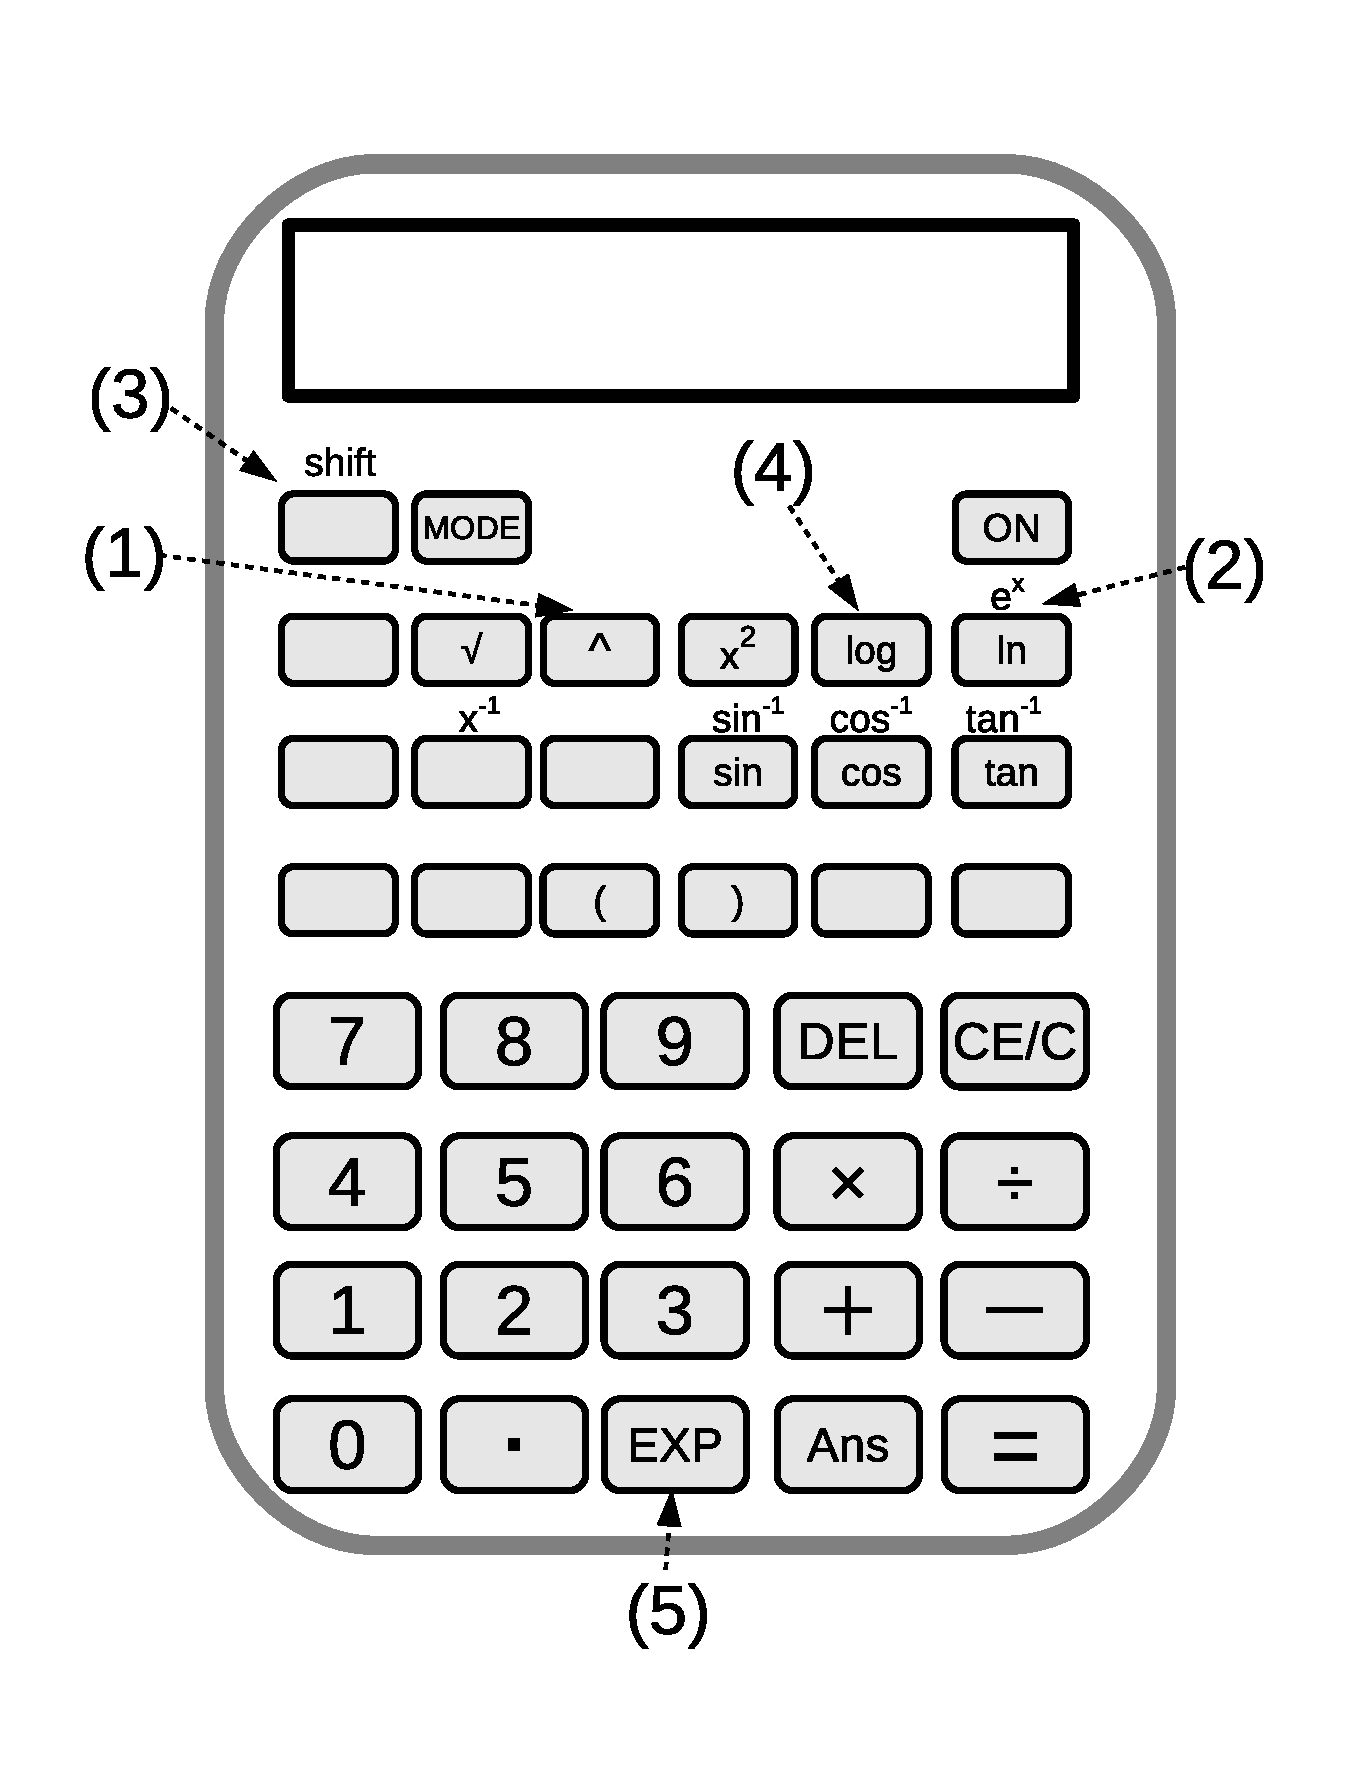
\includegraphics[width=7.5cm]{calculator.eps}
    \caption{関数電卓。普通の電卓と違って, キーがたくさん
ある。特に, (2)や(4)のキーがあるところが, 普通の電卓との違い。}\label{fig:calculator}
\end{figure}
ここでは, 例として, 
$2.3^{4.5}$を求めてみよう。

まず, 数字キーを使って2.3と
入れる。次に, 図\ref{fig:calculator}の(1)で示した, 「$\hat{\,}$」という
キーを押す(計算機の業界では, 「$\hat{\,}$」は累乗を意味する。なお, 
製品によっては, 「$\hat{\,}$」が無いものもある。その場合は, かわりに
「$x^y$」というキーを押す)。そして再び数字キーで4.5と入れる。
最後に, 右下の「=」ボタンを押そう。すると, 42.43998$\cdots$という答が
表示されるだろう。

\begin{q}\label{q:alg_dentaku2} 
以下の数を電卓で小数第5位まで求めよ。
\begin{edaenumerate}<3>
\item $2^{3.5}$
\item $1.01^{100}$
\item $\sqrt[3]{5}$
\end{edaenumerate}
ヒント: 3乗根は, 1/3乗, つまり, 0.3333333...乗。
\end{q}
\mv

\section{ネイピア数}

さて, ちょっと唐突だが, 大学では「ネイピア数」\index{ねいぴあすう@ネイピア数}
というものが頻出する。ネイピア数は無理数であり, 慣習的に$e$という記号で表す。その値は,  
\begin{itembox}{ネイピア数}
\begin{eqnarray}
e=2.71828\cdots\label{eq:NapierNum_value}
\end{eqnarray}
\end{itembox}
である(これは定義ではない。ネイピア数の定義は第\ref{chapt_exp_log}章で学ぶ)。
これには「似てないやつ」「フナひと鉢ふた鉢」等の語呂合わせがある。
この値を, 少なくとも4桁めまでは記憶せよ。\hv

\begin{q}\label{q:Napier_value_memorize} \eref{eq:NapierNum_value}
を10回書いて, 記憶せよ。\end{q}

$e$は, 数学において, $\pi$と同じくらいに重要な数だ。なぜ, どのように重要
なのかは, 後の章で学ぶ。

$x$を任意の実数として, ネイピア数の$x$乗, すなわち, $e^x$のことを, $\exp x$
と書くこともある。これも大切なことなので, 必ず記憶しよう:
\begin{itembox}{約束}
$\exp x$とは, $e^x$のこと。
\end{itembox}

関数電卓で$e^x$を求めるときは, さっきやったように, 2.71828を「$\hat{\,}$」キーで
累乗してもいいのだが, もっと正確で簡単な方法がある: 
例えば$e^4$を求めるときは, 図\ref{fig:calculator}の(3)にある「Shiftキー」を押し, 
それに続いて(2)を押す\footnote{(2)のキーは本来はlnという機能なのだが(その意味は後ほど述べる), 
直前にShiftキーが押されていると, lnという機能ではなく, ボタンの上方に
書かれた$e^x$という機能に, 一時的に変わるのだ}。そして, 数字キーで4と入れて, 
最後に=キーを押せばよい。すると, 54.598$\cdots$という答が表示されるだろう。

ただし, 製品によっては, この手順を若干, 入れ替える必要がある。すなわち, 
まず4を入れて, その後で, Shiftキー, (2)のキー(lnキー), という順序でないと
ダメなものもある。いろいろ試してみよう!

ちなみに, 電卓には図\ref{fig:calculator}の(5)のように, EXPというキーも
ある。しかし, これは, $e^x$ではないことに注意!

\begin{q}\label{q:alg_dentaku_exp} 
以下の数を電卓で小数第5位まで求めよ。
\begin{edaenumerate}
\item $\exp 2$
\item $e^{-1.5}$
\end{edaenumerate}
\end{q}

\begin{faq}{\small\textgt{関数電卓の使い方がわかりません} ... 関数電卓は
機種によって機能やデザインが違います。とりあえず, 間違えることを
恐れないで, いろいろ遊んでみよう。また, ネットで「関数電卓の使い方」
で検索してみよう。どうしてもわからなければ, 質問においで!}\end{faq}


\section{対数}

正の実数$a, b$について, 「$a$を何乗すると$b$になるか」の指数を求める
操作($a^x=b$となるような$x$を求める操作)を, 
\begin{eqnarray}
\log_a b\label{eq:taisuu00}
\end{eqnarray}
とあらわす(ただし, $a\neq 1$とする)。これを
\index{log}\underline{対数}\index{たいすう@対数} (logarithm)とよぶ(定義)
\footnote{ここで$a, b$は正としたが, これらが負であっても, 同様のことを考えることは, 
場合によっては可能である。例えば$b=-8$, $a=-2$とすれば, 「$a$を何乗すると$b$になるか」の答えは
3である。しかし, 例えば$b=8, a=-2$とか, $b=-8, a=2$とかになると, $a$を何乗しても$b$にはならない。
このような例外がたくさん生じるのは面倒なので, 対数を考えるときは, 普通, $a$や$b$に相当する数を
プラスに限定するのだ。}。\eref{eq:taisuu00}の$a$にあたる数を\underline{底} \index{てい@底}と呼ぶ。\eref{eq:taisuu00}の$b$にあたる数を\underline{真数} \index{しんすう@真数}と呼ぶ。

\begin{exmpl} 
\begin{itemize}
\item $\log_2 8=3$である。2を3乗したら8になるから。
\item $\log_2 1=0$である。2を0乗したら1になるから。
\item $\log_2 0.5=-1$である。2を$-1$乗したら1/2, つまり0.5になるから。
\end{itemize}
%(例おわり)
\end{exmpl}

\begin{q}\label{q:exp_logvalue0} 以下の値を求めよ(電卓等を使わずに):
\begin{edaenumerate}<3>
\item $\log_2 4$
\item $\log_{3} 81$
\item $\log_{0.1} 0.01$
\item $\log_{10} 1000$
\item $\log_{10} 0.01$
\item $\log_{10} 1$
\end{edaenumerate}\end{q}
\hv

10を底とする対数を\underline{常用対数} \index{じょうようたいすう@常用対数}と呼ぶ。
また, ネイピア数$e=2.718\cdots$を底とする対数を\underline{自然対数} \index{しぜんたいすう@自然対数}
と呼ぶので, ネイピア数のことを「自然対数の底」\index{しぜんたいすうのてい@自然対数の底}と
呼ぶことも多い。

\begin{q}\label{q:whatis_log} 以下の言葉の定義を述べよ:
\begin{edaenumerate}
\item 対数
\item 常用対数 
\item 自然対数
\end{edaenumerate}
\end{q}

常用対数や自然対数はよく使うので, 底を省略して$\log x$と書かれることが
世間ではよくある。その場合, 常用対数なのか自然対数なのか, 
読者が空気を読んで判断しなければならない。これはトラブルの種
であり危険な慣習である。君はこんな慣習を真似てはダメ。
常用対数なら, 面倒くさがらずに$\log_{10}x$と書くべし。一方, 
自然対数は, $\ln x$\index{ln}と書く慣習もある。lnはlog natural
の略である。これは底を誤解する余地が無く, 便利なので, 我々はこの表記を採用しよう。
\begin{itembox}{約束}
対数の底を省略しない。つまり, 常用対数や自然対数を, 
$\log x$と書いてはいけない。自然対数($\log_e x$のこと)は
$\ln x$と書いてもよい。
\end{itembox}

生物資源学類「基礎数学I, II」「物理学I」等では, 上の
「約束」を守らない答案は, \textgt{全て零点!}

\begin{freqmiss}{\small\textgt{自然対数lnをInとか1nと書いてしまう} ...
lは小文字のエルです。数字のイチや, 大文字のアイでは
ありません。手書きのときは, 筆記体($\ell$)で書こう!}\end{freqmiss}

\begin{faq}{\small\textgt{高校数学では, 自然対数は$\log x$でOK
でした。大学の他の授業や教科書も, $\log x$と書いてるのは多いです。
$\log x$と書いたら零点なんてキツすぎません?} ... 
こういう例があります: 森林科学では, 木の体積(それが木材としての商品価値を決める!)を, 
木の高さと胸高直径(人の胸の高さで測った幹の直径)で推定します。
ある論文で, その推定式が, 対数を使って書かれていましたが, 
底が省略されており, それが10なのか$e$なのか, わかりませんでした。
君ならどうしますか? 10か$e$のどちらかを適当に使いますか? 
それで間違った計算をして, まだ十分に大きくなっていない木を
切っちゃったらどうします? あるいは, 君の書く論文で対数の底が
書いてないせいで, 誰かがそういうミスをしたら, どうします?
}\end{faq}

関数電卓で自然対数を求める時は, lnというキーを使う(図\ref{fig:calculator}の(2))。
例えば, $\ln 3$を知りたかったら, lnキーを押して, その後に3を押し, =キーを押せば
よい。製品によっては逆のこともある。つまり, 先に3を押し, そのあとでlnキー, という
場合もある。

同様に, 常用対数を求める時は, logというキーを使う(図\ref{fig:calculator}の(4))。
多くの関数電卓では, logは常用対数を意味する。例えば, $\log_{10} 2$を
知りたかったら, logキー, 2, =を順に押せば良い(もしくは, 2, logキーの順)。

\begin{q}\label{q:alg_dentaku_ln} 
電卓を使って以下を小数第5位まで求めよ。\\
(1) $\log_{10} 2$ 
(2) $\log_{10} 0.006$ 
(3) $\ln 2$ 
(4) $\ln 10$
\end{q}
\mv


\section{ベクトル}\label{sect:vector_digest}

平面や空間の中で, 大きさと向きをもつ量(速度とか力とか)を
\underline{ベクトル} \index{べくとる@ベクトル}と呼ぶ。ベクトルは
物理学や化学に関連した授業で頻繁に出てくるので, ここで基本
を学んでおこう。

ベクトルは矢印で図示する。「大きさ」を
矢印の長さで表現し, 「向き」を矢印の向きで表現するのだ。

ベクトルが空間の中のどこにあるか, ということは考えない(というか, 問題にしない)。
例えば, 風速1.0~m~s$^{-1}$の風が北から南向きに吹く, という現象(風速)を
ベクトルとして表現すると, その風がどこの場所で吹いているか, ということは問題
にしない。従って, 以下に描いた3つのベクトルは, いずれも互いに等しい
ベクトルである(描かれた場所は違っても, 矢印の長さと向きは同じだから)。

\begin{center}
\setlength{\unitlength}{1mm}
\begin{picture}(60,15)
\thicklines
\put(2,8){\vector(2,1){10}}
\put(18,1){\vector(2,1){10}}
\put(36,10){\vector(2,1){10}}
\end{picture}
\end{center}

数を$a$や$x$のような記号で表すように, ベクトルも記号で表すことが多い。高校数学では
\begin{eqnarray*}\overrightarrow{a}, \overrightarrow{b}, \overrightarrow{c}, \cdots, \overrightarrow{x}, \overrightarrow{y}, \overrightarrow{z},
\overrightarrow{A}, \overrightarrow{B}, \overrightarrow{C}, \cdots, \overrightarrow{X}, \overrightarrow{Y}, \overrightarrow{Z}\end{eqnarray*}
のように, 矢印が上に載ったアルファベットで表す。しかし大学では, 
\begin{eqnarray*}{\bf a}, {\bf b}, {\bf c}, \cdots, {\bf x}, {\bf y}, {\bf z}, 
{\bf A}, {\bf B}, {\bf C}, \cdots, {\bf X}, {\bf Y}, {\bf Z}\end{eqnarray*}
のように, 太字のアルファベットで表すことが多い。手書きすると図\ref{fig:vector}のようになる。

\begin{figure}\centering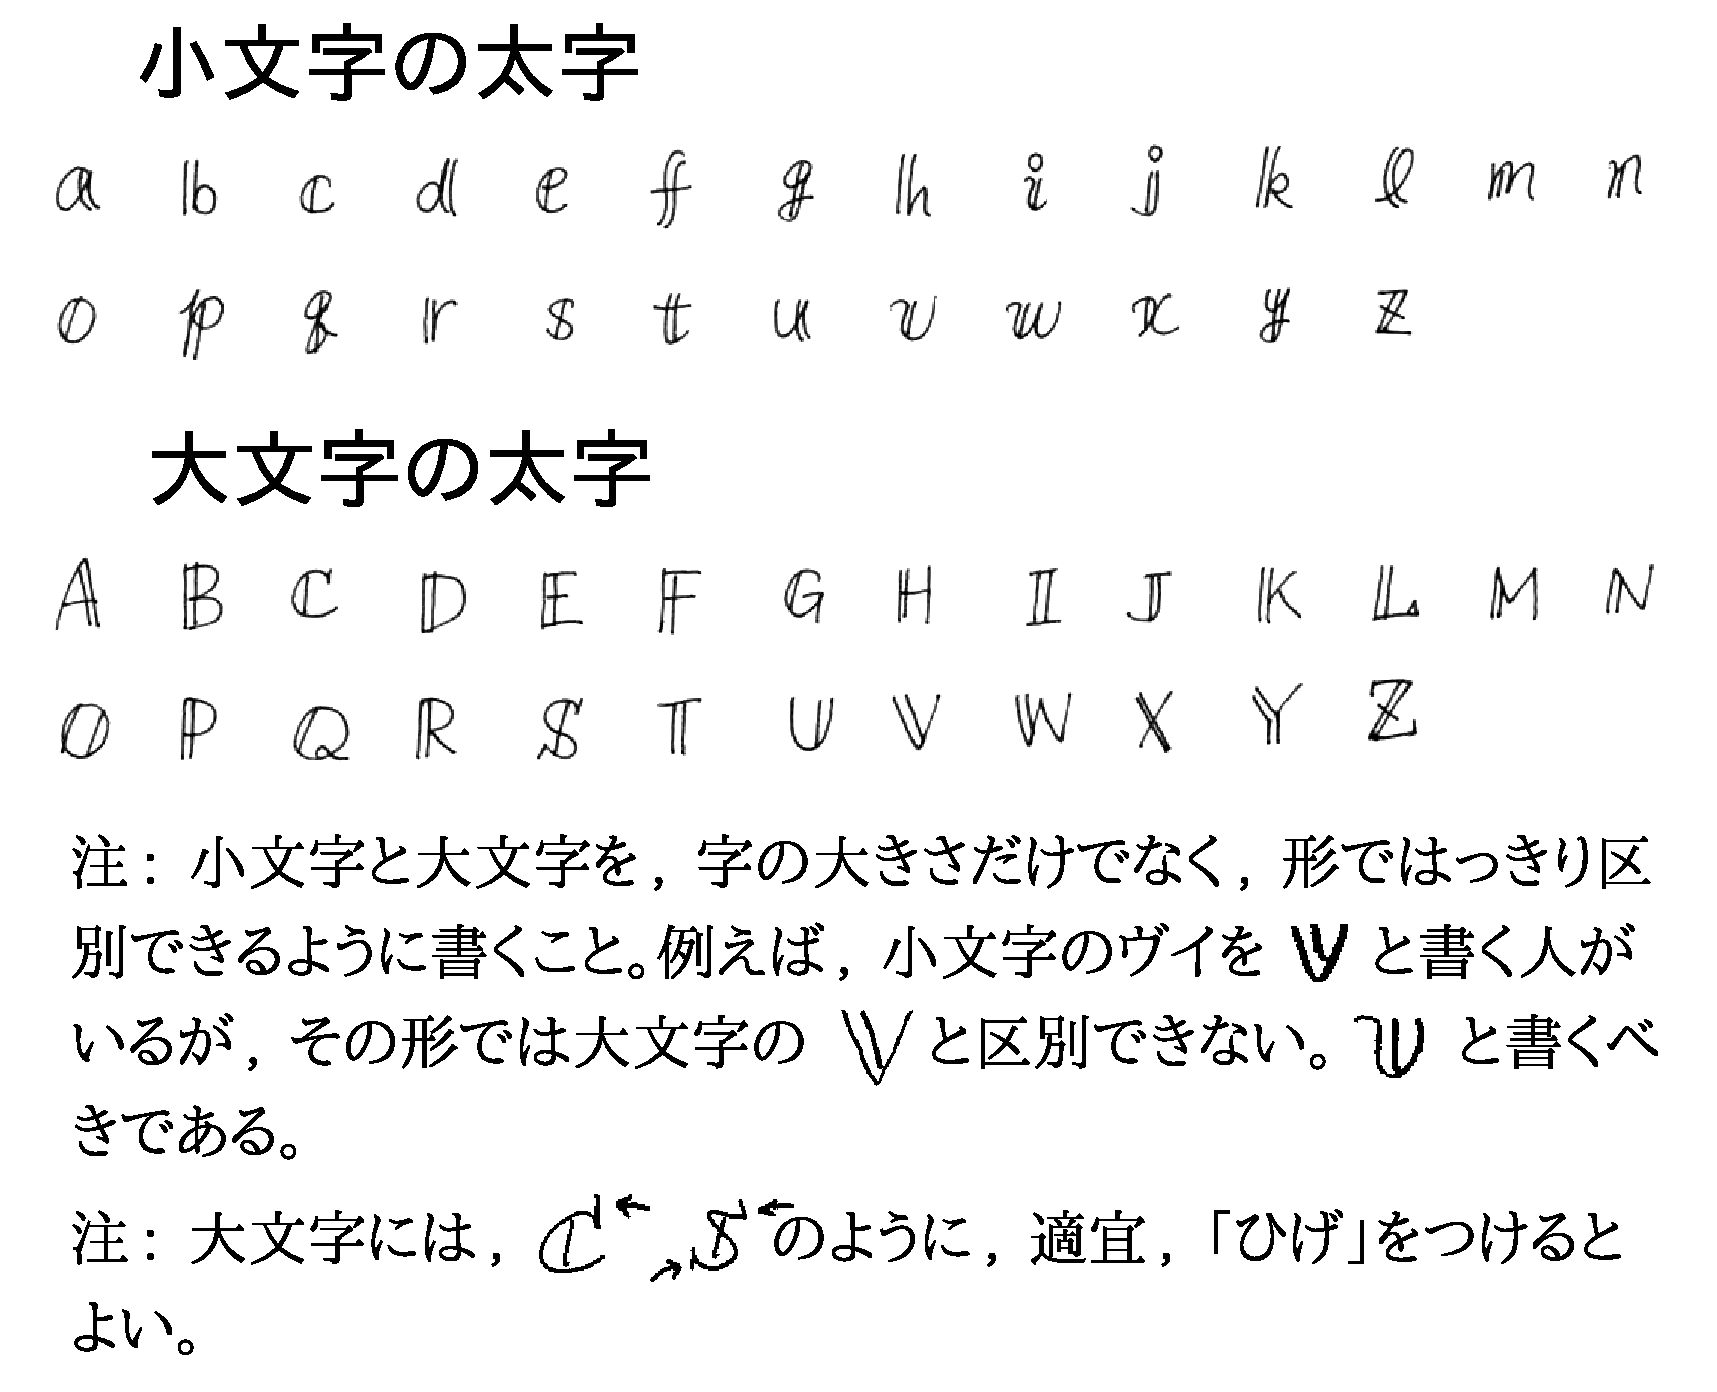
\includegraphics[width=8.0cm]{futoji.eps}

\caption{太字のアルファベットの手書き例。大切なのは, 1:太字だとわかること, 2:何の字かわかること, 
3:大文字と小文字を形で区別できること。この3つを全て満たしていれば, どう書いてもかまわない。
特に3について, 注意が必要なのは, ${\bf C}$と${\bf c}$, ${\bf O}$と${\bf o}$, ${\bf P}$と${\bf p}$, 
${\bf S}$と${\bf s}$, ${\bf V}$と${\bf v}$, ${\bf W}$と${\bf w}$, ${\bf X}$と${\bf x}$, 
${\bf Z}$と${\bf z}$である。また, ${\bf h}$と${\bf n}$も容易に紛らわしくなるので
注意。\label{fig:vector}}
\end{figure}

\begin{q}\label{q:vect_write} 図\ref{fig:vector}を参考にして, 
太字のアルファベットを全て(小文字・大文字ともに), 3回ずつ書け。\end{q}

ベクトルを記号で表すやりかたとして, もうひとつ便利なのがある。下図のように
空間に点A, Bがある場合...
\begin{center}
\setlength{\unitlength}{1mm}
\begin{picture}(40,13)
\put(2,2){\circle*{2}}
\put(31.5,11.9){\circle*{2}}
\put(30,14.5){B}
\put(1,5){A}
\thicklines
\put(2,2){\vector(3,1){29}}
\put(12,9){$\overrightarrow{\text{AB}}$}
\end{picture}
\end{center}
点Aを始点とし, 点Bを終点とするようなベクトルを扱いたいことが
よくある。そういうとき, そのベクトルを$\overrightarrow{\text{AB}}$
と書くのだ。\mv

\begin{faq}{\small\textgt{さっき, 「ベクトルが空間の中の
どこにあるか, ということは考えない」とありましたよね。でも, 
そのベクトル$\overrightarrow{\text{AB}}$は, 点Aと点B (の間)
にあります。なんか矛盾してません?} ... 確かに$\overrightarrow{\text{AB}}$は
特定の場所A, Bを使って定義されましたが, それをどの場所に持って行っても
いいのです。例えばもしも別の場所に点Cと点Dがあって, $\overrightarrow{\text{CD}}$
が$\overrightarrow{\text{AB}}$と同じ向きで同じ大きさ(長さ)なら 
$\overrightarrow{\text{AB}}=\overrightarrow{\text{CD}}$なので, 
$\overrightarrow{\text{CD}}$のことを$\overrightarrow{\text{AB}}$と
呼んでもいいのです(紛らわしいけど間違いではない)。}\end{faq}

ベクトル${\bf a}$の大きさを$|{\bf a}|$と表す。大きさが0であるような
ベクトルを${\bf 0}$と書く。すなわち$|{\bf 0}|=0$である。\\

さて, 「向きを持たず, 大きさだけを持つ量」を\underline{スカラー} 
\index{すからー@スカラー}
% (scalar)
と呼ぶ。要するに普通の実数(2とか3.14とか$-5$など)のことだ。

\begin{faq}{\small\textgt{なら, スカラーなんて言葉を使わないで, 
単に実数と呼べばいいじゃないですか?} ... それはそうですが, 
「ベクトルでない量」という意味合いを含ませるためにあえて
スカラーと呼ぶのです。}\end{faq}

$\alpha$をスカラー, ${\bf a}$をベクトルとする。${\bf a}$と同じ向きで
大きさが$\alpha$倍であるようなベクトルを, 「ベクトル${\bf a}$の$\alpha$倍」, 
もしくは$\alpha {\bf a}$と定義する。ただし, マイナス倍は, 向きを逆にする。

\begin{center}
\setlength{\unitlength}{1mm}
\begin{picture}(60,12)
\thicklines
\put(2,5){\vector(2,1){10}}
\put(5,10){${\bf a}$}
\put(18,3){\vector(2,1){20}}
\put(24,9){$2 {\bf a}$}
\put(56,10){\vector(-2,-1){10}}
\put(46,9){$- {\bf a}$}
\end{picture}
\end{center}

スカラーを表す変数は, 普通の数の変数と同じように, 細字の
斜字体で表記する。スカラーとベクトルの表記の違いをよく見比べてみよう:
\begin{itembox}{スカラーとベクトルの字体の違い}
スカラー: $a, b, c,\, \cdots,\, x, y, z, A, B, C,\, \cdots,\, X, Y, Z$\\
ベクトル: ${\bf a}, {\bf b}, {\bf c}, \cdots, {\bf x}, {\bf y}, {\bf z}, 
{\bf A}, {\bf B}, {\bf C}, \cdots, {\bf X}, {\bf Y}, {\bf Z}$
\end{itembox}
両者は見た目で明らかに違う。字の太さだけでなく, 形も違う。
この違いをよく覚えて, スカラーとベクトルを混同しないようにして欲しい。\\

\begin{freqmiss}{\small\textgt{ベクトルを普通の(矢印もつけない)細字, 
つまり$a, b, c, \cdots$等と書いてしまう} ... 
これは, 毎年, 多くの資源生が何回も何回もやらかします。あまりに深刻なので, 
大きく書いておこう!}\end{freqmiss}
\begin{itembox}{約束}
ベクトルは太字で書くか, 上付き矢印を書くこと! \textgt{単なる細字で書いてはいけない}!
\end{itembox}
%印刷物やプリントを, 注意して見よう。
%太字と細字が明確に区別されて使われていることがわかるだろう。

また, 太字で書くと決めたベクトルを上付き矢印で書いたり, その逆をしたりしてはいけない。
例えば, あるベクトルを${\bf a}$と書くと決めたなら, それを$\vec{a}$と書いてはいけない。\\

2つのベクトル${\bf a}$, ${\bf b}$が, 0でないスカラー$\alpha$によって, 
\begin{eqnarray}
\alpha{\bf a}={\bf b}\label{eq:def_parallel}
\end{eqnarray}
と書けるとき, ${\bf a}$と${\bf b}$は互いに\underline{平行}\index{へいこう@平行}
である, という(定義)。これは直感的に明らかだろう。\\

ここで, ベクトル同士の足し算(和)を定義しよう: 2つのベクトル${\bf a}$, ${\bf b}$について, 
${\bf a}$の終点に${\bf b}$の始点を置いたときに, ${\bf a}$の始点から${\bf b}$の終点まで
を結ぶベクトルを, 「${\bf a}$と${\bf b}$の和」, もしくは${\bf a}+{\bf b}$と定義する。

\begin{center}
\setlength{\unitlength}{1mm}
\begin{picture}(60,18)
\thicklines
\put(11,15){\vector(1,0){20}}
\put(18,17){${\bf b}$}
\put(2,5){\vector(1,1){10}}
\put(4,10){${\bf a}$}
\put(2,5){\vector(3,1){29}}
\put(16,8){${\bf a}+{\bf b}$}
\end{picture}
\end{center}
または, こう考えても良い:${\bf a}$, ${\bf b}$の各始点を共有させるときに, 
${\bf a}$, ${\bf b}$が張る平行四辺形の対角線(始点は各ベクトルの始点)に対応するベクトルが, 
${\bf a}+{\bf b}$である。中学校の理科でやった, 平行四辺形を使った力の合成を思い出せばよい。

\begin{center}
\setlength{\unitlength}{1mm}
\begin{picture}(60,20)
\thicklines
\put(2,10){\vector(1,0){20}}
\put(12,6){${\bf b}$}
\put(2,10){\vector(1,1){10}}
\put(4,15){${\bf a}$}
\put(2,10){\vector(3,1){29}}
\put(16,13){${\bf a}+{\bf b}$}
\thinlines
\put(11,20){\line(1,0){20}}
\put(22,10){\line(1,1){10}}
\end{picture}
\end{center}
これらの2つの考え方(定義)は, 同等である。

\begin{q}\label{q:vect_add_fig} 以下の2つのベクトル${\bf a}, {\bf b}$について, ${\bf a}+{\bf b}$, ${\bf a}-{\bf b}$, $2{\bf a} + 3{\bf b}$
を, それぞれ作図せよ。
\begin{center}
\setlength{\unitlength}{1mm}
\begin{picture}(60,19)
\thicklines
\put(27,10){\vector(2,-1){15}}
\put(37,6){${\bf a}$}
\put(12,10){\vector(1,1){10}}
\put(14,15){${\bf b}$}
\end{picture}
\end{center}
\end{q}
\mv

次に, ベクトル同士の引き算(差)を定義しよう: 2つのベクトル${\bf a}$, ${\bf b}$について, 
\begin{eqnarray*}
{\bf a}={\bf b}+{\bf x}\quad\text{を満たすベクトル${\bf x}$を求めること}
\end{eqnarray*}
を「{\bf a}から{\bf b}を引く」と呼び, ${\bf a}-{\bf b}$と書く。これは, 形式的には
\eref{eq:def_subtract}とほとんど同じだ。図では以下のようになる:

\begin{center}
\setlength{\unitlength}{1mm}
\begin{picture}(60,22)
\thicklines
\put(20,10){\vector(2,-1){15}}
\put(25,3){${\bf b}$}
\put(20,10){\vector(1,1){10}}
\put(22,15){${\bf a}$}
\put(35,4){\vector(-1,3){5}}
\put(35,10){${\bf a} - {\bf b}$}
\end{picture}
\end{center}

初心者はこの話で, ${\bf a}-{\bf b}$の向きを混乱することがよくある。
${\bf a}-{\bf b}$の終点は${\bf a}$(の終点)であり, 
${\bf a}-{\bf b}$の始点は${\bf b}$(の終点)である。
これを縮めて, 「ベクトルの引き算は終点引く始点」と覚えるとよい。\\

さて, ベクトルを表す時にいつも矢印を作図するのは面倒くさくて仕方ない。
そこで便利なのが「座標」という考えである。これは, \fref{fig:vector_coordinate}
のように, ベクトルを座標平面($x$軸と$y$軸があるような平面)の
上に, 始点が原点Oに来るように\footnote{原点をあらわすOは「零」ではない。
originの頭文字の「オー」の大文字である。}置き, 終点(矢印の先端)から$x$軸と
$y$軸のそれぞれに垂直に線をおろして(方眼紙のように), 
原点からそれぞれへの長さを, $(3, 2)$のように並べたものである。

\begin{figure}
    \centering
    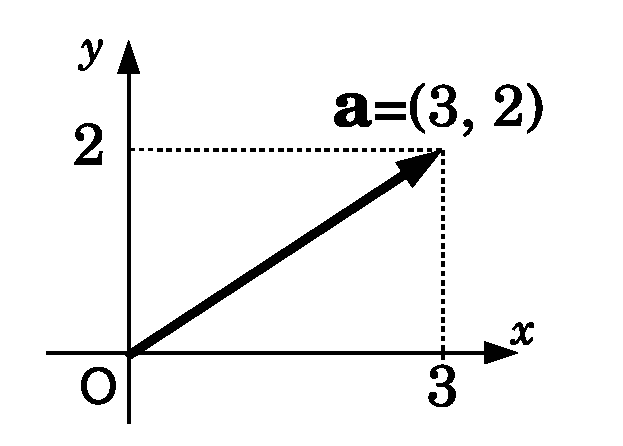
\includegraphics[width=4cm]{vector_coordinate.eps}
    \caption{ベクトルを座標で表す。\label{fig:vector_coordinate}}
\end{figure}

これは平面上のベクトルの場合だが, 空間のベクトルの場合は, さらに
高さ方向の軸($z$軸)があるような座標空間を考えて, $(3, 2, 1)$のように
3つの数値を並べることで表現できる。こういうのを「座標」と呼ぶ。
ベクトルは矢印で表しても, 座標で表してもよいのである。\\

座標の利点は, 「計算が楽」ということだ。あるベクトルをスカラー倍したり
ベクトル同士を足したり引いたりするとき, 矢印ならいちいち作図しなければ
ならないが, 座標なら数値の計算で済む。

\begin{exmpl} ${\bf a}=(1, 2)$と${\bf b}=(-3, 4)$について, 
$5{\bf a}+{\bf b}$は?\\
$5{\bf a}+{\bf b}=5(1, 2)+(-3, 4)=(5\times1-3, 5\times2+4)=(2, 14)$
(例おわり)\end{exmpl}

\section{位置ベクトル}

前述したように, ベクトルは大きさ(長さ)と向きを持つ量であり, 本来は, 
それが空間のどこにあるかは問わない。でも, 空間内のどこかに原点O
を定めれば, 空間内の点Pの位置は, ベクトル$\overrightarrow{\text{OP}}$
によって表現できる。このように, 空間の点の位置を表すベクトルのことを, 
\underline{位置ベクトル} \index{いちべくとる@位置ベクトル}という。
位置ベクトルを考えるときは, 空間内のどこかに原点があって, そこを始点とするベクトルを
考えているのだという意識を持とう。ただし, その原点が具体的にどこなのかは, 
多くの場合は問題にされない。どこかは知らなくても, どこかにあるのだ。

位置ベクトルは, 次の例のように使う:

\begin{exmpl} 空間内に2つの点A, Bがあり, それぞれの位置ベクトルを${\bf a}$, ${\bf b}$
とする。その意味は, どこかに適当な原点Oがあって(どこでもよい), ${\bf a}=\overrightarrow{\text{OA}}$, 
${\bf b}=\overrightarrow{\text{OB}}$である, ということだ。このとき, 
$\overrightarrow{\text{AB}}={\bf b}-{\bf a}$である(なぜかは各自
考えてみよう)。また, 線分ABの中点Cの位置ベクトル${\bf c}$は(${\bf c}$は
$\overrightarrow{\text{OC}}$のこと), 
\begin{eqnarray}
{\bf c}=\frac{{\bf a}+{\bf b}}{2}\label{eq:vect_middlepoint}
\end{eqnarray}
である(なぜかは各自考えてみよう)。

では, 線分ABを$m:n$に内分\index{ないぶん@内分}する点P (つまり, 線分AB上にあって, 
AP:PB$=m:n$になるような点P)は, どこにあるだろうか? Pの位置ベクトルを$\bf p$
としよう(図\ref{fig:vector_3})。明らかに, 
\begin{eqnarray}
{\bf p}&=&\overrightarrow{\text{OA}}+\overrightarrow{\text{AP}}={\bf a} + \frac{m}{m+n}\overrightarrow{\text{AB}}={\bf a} + \frac{m}{m+n}({\bf b}-{\bf a})\nonumber\\
&=&\frac{n {\bf a} + m {\bf b}}{m+n}\label{eq:vect_naibun}
\end{eqnarray}
となる。この式の右辺で$m=n=1$とすると\eref{eq:vect_middlepoint}の右辺に一致する!
\begin{figure}[h]
    \centering
    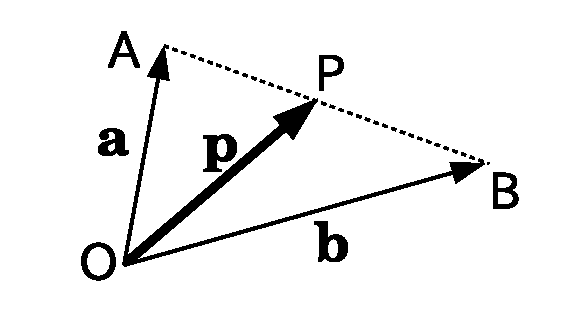
\includegraphics[width=4cm]{vector_3.eps}
    \caption{点Aと点Bの間を内分する点P。\label{fig:vector_3}}
\end{figure}
(例おわり)\end{exmpl}

\begin{q}\label{q:vect_pos2D} 点A, Bの位置ベクトルがそれぞれ(4, 5)と(3, 6)であるとき, 
\begin{enumerate}
\item ABを1:2に内分する点の座標を求めよ.
\item ABを2:1に内分する点の座標を求めよ.
\end{enumerate}\end{q}\mv


\begin{faq}{\small\textgt{ベクトルは太字よりも
上付き矢印を使ったほうが分かりやすいです。}
... そのうち太字に慣れますよ。}\end{faq}

\begin{comment}
ここで書き方に関する注意。問\ref{q:vect_pos2D}のように, A(1, 2)と
書くときは, Aは点の名前(ラベル)であり, (1, 2)は点の座標である。
そして, この点の位置ベクトルを${\bf a}$とすると, ${\bf a}=(1, 2)$
と書く。ところが, これを, ${\bf a}(1, 2)$と書く人がいる。\textgt{これはよくない}。
${\bf a}$と$(1, 2)$の間には, 必ず等号を書かねばならない。
というのも, 
数学では, ${\bf a}(1, 2)$は${\bf a}=(1, 2)$とは違った意味を持つ
のである\footnote{平面上の全ての点にひとつずつベクトルが存在する
ような数学的概念を考えると, それは${\bf a}(x, y)$のように表される。
その場合, 点(2, 3)\textgt{における}ベクトルを${\bf a}(2, 3)$
のように表す(これはちょうど, 関数$f(x)$について, $x=4$での
値が$f(4)$である, というのと同じような括弧の使い方である)。
このとき, (2, 3)は, そのベクトルがある場所を表すのであり, 
そのベクトルそのものを表すのではない。だから, もしかしたら
${\bf a}(2, 3)=(1, 2)$かもしれないし, ${\bf a}(2, 3)=(0, 0)$
かもしれない。}。
\end{comment}
\mv



\section{有効数字}

現実的な話題で出てくる数値の多くは, 誤差を持つ。

例えば, 総務省統計局によると, 平成27年2月1日現在, 日本の総人口は, 
「1億2697万人」らしい。この推計値に「1万人」の桁までしかないことに
注意しよう。本当は, 1億2697万5678人とか, 1億2697万1212人
のように, 万よりも小さな桁にも何か数があるはず。でも, 誤差のために, 
そこまでの詳しい数は出せないのだ。というのも, 日本では, 1日に約3千人
(約30秒に1人)のペースで赤ちゃんが生まれるし, 同じくらいのペース
で人が亡くなっている。それらの人の生死は等間隔で起きるわけではないし, 
起きてすぐに総務省に報告が来るわけでもないから, 誤差ゼロで
人口を推計することはほぼ無理だし, 意味ないのだ。

そこで, 上の「1億2697万」という数は, 億から万までの位の数字, 
つまり, 1, 2, 6, 9, 7だけが意味あると考える。このように, 
誤差を含む数値において, 意味のある数字のことを
「有効数字」\index{ゆうこうすうじ@有効数字}と呼ぶ。そして誤差は, 
有効数字の中で, 最も小さな位の数(上の例では7)に影響する程度
だろうと考える。従って, 最も小さな位の数は, 信用できない(意味がない)
わけではないが, ちょっと怪しいぞ(上の例では, 7が6とか8になってもおかしく
ないかも), と疑ってかかるのだ(つまり, 怪しい数字の最大の位が
有効数字の最小の位である)。\\

誤差のある数値を扱う時は, 常に有効数字を意識しよう。まず, 
数値の有効数字がどの桁までなのかをはっきりさせよう。
そのときに注意が必要なのは「0」という数字の扱いである。

例えば, 「A君, 今, いくら持ってる?」という問に, A君が「だいたい1200円」
と答えたとする。このとき, おそらく真実は1100円から1300円くらい
の間にある(誤差は100円くらい)と考えるのが常識的な判断だろう。この場合, 
有効数字は1と2の2桁であり, それよりも下の2桁の0は, 有効数字ではなく, 
位取りのため(数値の桁を表現するため)の0であるにすぎない。ところが, 
A君は実際は几帳面な人で, 10円単位で財布の中身を把握
していたとするなら, A君の「だいたい1200円」
の意味するところは, 1190円から1210円くらい, ということになる。その場合, 
1, 2だけでなく, その次の0(つまり10円の位の0)も, 有効数字である。

つまり, 0という数字は困ったもので, 「位取りの0」と「有効数字の0」という
2つの異なる役割を担う。それが紛らわしくて, 数値を見ただけでは判断
できないのだ(そういう意味では, 上の人口の「1億2697万人」
の例でも, ホントは有効数字の0が万よりも小さな位, 例えば千とか
百にもあったかもしれない)。

ところが, 小数点が現れると, 有効数字がはっきりすることがある。例えば, 
100.0という表現を考えよう。これは数学的には100と同じ。
だから, 100.0なんて書かずに, 100と書けば良いように思う。
実際, 小数点より右側には, 位取りのために末尾(右端)に0を付け加える
必要は無い。にもかかわらず, わざわざ100.0というふうに小数点の右側
に0がある場合, この0は位取りの0ではなく, 有効数字の一部であると
解釈するしかない。すると, それよりも大きな位の数は, 全部有効数字の
はずである。従って, 100.0は, 1, 0, 0, 0という4つの数が有効数字
である, つまり有効数字は4桁である, と自信を持って判断できるのだ。
ところが, 単に100と表していたら, 自信を持って有効数字であると
判断できるのは最初の1だけだ。

では例えば, 0.0012の有効数字はどれだろうか? 1, 2は当然, 有効数字である。
しかし, それより上位にある3つの0は, 小数の位取りを表す0と考えるのが
適当である。従って, 0.0012の有効数字は, 1と2の2桁である。\\

\begin{q}\label{q:guard_digit_order} 以下の数のそれぞれについて, 
有効数字を指摘せよ。
\begin{edaenumerate}<4>
\item $5.3$
\item $1230.5$
\item $5300$
\item $0.0230$
\end{edaenumerate}
\end{q}

このように, 有効数字は, 表現法によっては曖昧になってしまう。
有効数字をはっきりさせたいときは, 数値をあえて小数を使って
書く。つまり, 小数×「10の累乗」の形で書くのである。例えば, 1200円を, 
\begin{eqnarray}
1.2\times10^3\,\text{円}\label{eq:1200yen3}\\
\text{とか, }\nonumber\\
1.20\times10^3\,\text{円}\label{eq:1200yen4}
\end{eqnarray}
というふうに書くのだ。\eref{eq:1200yen3}の場合は有効数字は1と2だけ(100円の位まで意味がある)
だが, \eref{eq:1200yen4}の場合は有効数字は1, 2, 0となる(10円の位まで意味がある)。
数学的には, $1.2\times10^3$と$1.20\times10^3$は同じなのだが, 
現実世界において誤差を含む数としては, これらは別物なのである。\\



\section{有効数字の計算}

では, 有効数字を計算(四則演算)の中でどのように扱うかを述べる。

例として, 4.56と1.2という数値の和を考える。それを筆算でやってみよう。
その際, 「怪しい数」を以下のように追跡する: まず, 
4.56は有効数字3桁で, 最後の6がちょっと怪しいのでその6を○で囲って
おこう。1.2は有効数字2桁で, 最後の2がちょっと怪しいのでその2を
□で囲っておこう。さて, 怪しい数が足されて得られた数は, 怪しさが
「伝染」してくるはずなので, その数も, ○または□で囲う。どちらの形で
囲うかは, その怪しさが伝染してきたもとの数を囲う形で決める。
ただし, 怪しい数からの繰り上がりによって受ける影響は
無視する(怪しくないとみなす)。

すると, 図\ref{fig:guard_digit_plus}のようになる:
\begin{figure}[h]
    \centering
    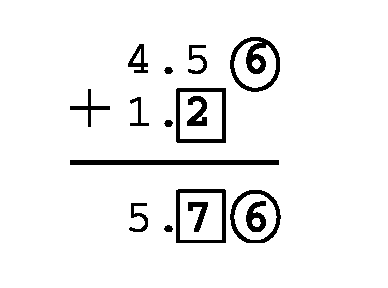
\includegraphics[width=3cm]{guard_digit_plus.eps}
    \caption{誤差を含む数どうしの和。怪しい数を○や□で囲って
ある。}\label{fig:guard_digit_plus}
\end{figure}

有効数字を考えなければ, 結果は5.76になる。最初の(1の位の)5は怪しくないが, その右(0.1の位)
の7は, 1.2の最小位の有効数字の怪しさの影響を受けているから, 怪しい。
この時点で, さらに右の6はあまり意味が無い。なぜなら, 0.1の位の7が, 
6とか8かもしれないなら, それよりも詳細な(桁の小さい)情報にこだわっても
仕方が無いからである。というわけで, この答の有効数字は, 最初の5と
次の7の2桁と考えるのが妥当だろう。そこで, 3桁目の6を切り捨てるか
切り上げよう。このように, 無意味な桁を切り捨てたり切り上げたりすることを
「丸める」\index{まるめる@丸める}という。多くの場合は, 四捨五入に
よって丸めるので, ここでは6を切り上げて最終的な答を5.8
としておこう。しかし, 「常に四捨五入が正しい」
というわけではなく, 場合によっては値によらず切り上げたり切り捨てたり
する方が妥当なこともある。

\begin{faq}{\small\textgt{「怪しい」とか「妥当だろう」とか「としておこう」
とか, なんかテキトーというか、いい加減なかんじですね。。。}
... そうです。後で述べるように, 有効数字というのは, テキトーでイイカゲン
なものなのです。}\end{faq}

このように, 足し算では, 最終的な答の有効数字は, 次のような手順で
決める: まず, 足す前の数の有効数字の最小(右端)の位をチェック。
上の例では「4.56」の右端は0.01の位であり, 「1.2」の右端は0.1の
位だ。次に, それらの中で, 最も大きな位に注目する。上の例では, 
0.1と0.01の比較となり, 大きいのは0.1の位である。その位を, 
最終的な答の有効数字の最小の位とする。上の例では, 5.76のうち, 
有効数字は0.1の位まで, つまり5と7が有効数字となる。そして, 
それより1つ小さな位を丸める。上の例では0.01の位の数, すなわち6を
四捨五入すると切り上がって, 5.8となる。こうして最終的な値を確定する。

ここでは詳しくは述べないが, 引き算も同様だ。引く数と引かれる数の
それぞれについて有効数字の最小位をチェックし, 最小位の大きい方を
最終結果の有効数字の最小位とし, それよりも1桁小さな数を丸めればよい。

\begin{q}\label{q:guard_digit_prac2} 以下の計算を行え。ただし, 
これらはいずれも誤差を含む数値とし, 有効数字に気をつけて, 無意味な
数を書かないように気をつけよ。電卓を使ってよい。丸めは四捨五入で行え。
\begin{edaenumerate}
\item $5.3 + 6.6$
\item $0.023 + 123.5$
\item $100.2 - 13$
\end{edaenumerate}
\end{q}

こんどは, 4.56と1.2の積を考えよう。それを筆算でやってみよう。
先ほどの和の例と同様に, 「怪しい数」を追跡する。すると, 
図\ref{fig:guard_digit_mult}のようになる:

\begin{figure}[h]
    \centering
    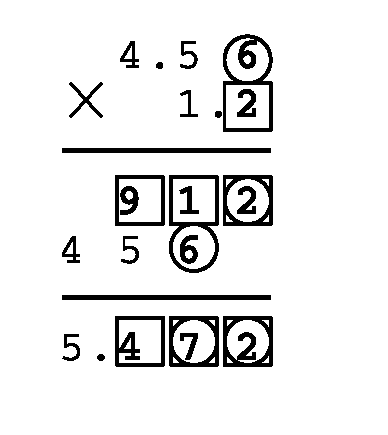
\includegraphics[width=3cm]{guard_digit_mult.eps}
    \caption{誤差を含む数どうしの積。怪しい数を○や□で囲って
ある。例えば, 3段目の9, 1, 2は, 右端の2が1段目の6の怪しさと
2段目の2の怪しさの両方の影響を
受けているので, ○と□の両方で囲ってある。}\label{fig:guard_digit_mult}
\end{figure}

有効数字を考えなければ, 結果は5.472になる。最初の(1の位の)5
は怪しくないが, その右(0.1の位)の4は怪しい。この時点で, 
さらに右の7や2はあまり意味が無い。なぜなら, 
0.1の位の4が, 3とか5かもしれないなら, それよりも詳細な(桁の小さい)
情報にこだわっても仕方が無いからである。

というわけで, この答の有効数字は, 最初の5と次の4の2桁と考えるのが
妥当だろう。そこで, 3桁目の7を切り捨てるか切り上げる。ここでは
四捨五入によって7を切り上げて最終的な答を5.5としておこう。

このように, 掛け算では, 最終的な答の有効数字は, 次のような手順で
決める: まず, 掛ける前の数の有効数字の桁数をチェックする。上の例
では「4.56」の3桁と, 「1.2」の2桁である。次に, それらの中で, 最も
小さな有効数字桁数に注目する。上の例では, 3桁と2桁の比較となり, 
最小は2桁である。その桁数を, 最終的な答の有効数字の桁数とする。
上の例では, 5.472のうち5と4の2桁が有効数字, となる。そして, 
最小の有効数字(上の例では4)よりも1桁小さな数値を丸め(上の
例では四捨五入の結果, 7が切り上がって4が5になる), 最終的な数を確定する。

ここでは詳しくは述べないが, 割り算も同様。割る数と割られる数の
それぞれについて有効数字の桁数をチェックし, 桁数の小さい方を最終結果
の有効数字の桁数とし, それよりも1桁小さな数を丸めればよい。

\begin{q}\label{q:guard_digit_prac4} 以下の計算を行え。ただし, 
これらはいずれも誤差を含む数値とし, 有効数字に気をつけて, 無意味な
数を書かないように気をつけよ。電卓を使ってよい。丸めは四捨五入で行え。
\begin{edaenumerate}
\item $5.3\times 2.6$
\item $0.023\times 123.5$
\item $100.2 / 13$
\end{edaenumerate}
\end{q}

\begin{exmpl} 長さ16 cmの棒を3等分したとき, 1本の長さは? 
小数で表せば, (16 cm)/3=5.333$\cdots$ cm。このとき, 
「16 cm」の有効数字は2桁なので, 結果の有効数字も2桁で
よかろう。3桁目を四捨五入し, 「5.3 cm」が妥当な答だろう。
 ... ちょっと待て! 「3等分」の「3」は有効数字1桁では? なら, 
結果も有効数字1桁, つまり「5 cm」が正しいのでは? と思った人
がいるかもしれない。でもそれは違うのだ。棒を3本に分けよ, 
と言われて「うっかり3.1本に分けちゃいました」なんてことは
あり得ない。つまり, この「3」の誤差は, 半端な小数ではなく, 
0, 1, 2などの整数のはず。でも, よほどのうっかり屋さんでも
3本を2本や4本に間違えることはなかろう。従って, この場合
の誤差は0。つまり, 「3本」は, 実は3.0000$\cdots$本, 
つまり有効数字が無限にある(小数点以下に有効数字の0が
無限に続く)と考えるのが妥当なのだ。従って, この割り算の
有効数字は, 「割られる数」である「16 cm」の有効数字の桁数
で決まるのだ。

ここで, 「小数にせずに, $\frac{16}{3}$ cmというふうに分数のまま
にしておけばいいじゃないか」と思う人もいるだろう。数学的にはそれで
正解である。でもこれが, 機械工作等の実務だったらどうだろうか? 
「$\frac{16}{3}$ cm」よりも「5.3 cm」の方が, ものさしで測りとる
のは簡単なので, 実務的な現場では, 数値は分数でなく
小数で表しておきたい, ということがよくあるのだ。(例おわり)\end{exmpl}



ここで注意。有効数字というのは, 実は, あまり厳密な考え方ではない。

\begin{exmpl} $3.47\times2.88$を考えよう。有効数字を考えなければ, \\
$3.47\times2.88=9.9936$\\
となる。3.47も2.88も有効数字3桁だから, 結果の有効数字は3桁のはず。
なので, 4桁目(3)以降を丸めて, 
$3.47\times2.88=9.99$\\
となる。ところが, この計算と微妙に違う, $3.47\times2.89$を考えよう。
有効数字を考えなければ, \\
$3.47\times2.89=10.0283$\\
となる。3.47も2.89も有効数字3桁だから, 結果の有効数字は3桁, ということで, 
4桁目以降(283)を丸めて, 
$3.47\times2.89=10.0$\\
となる。ここで, 変な気がしないだろうか? これらの2つの計算は, 
ほとんど同じような数値を扱っている(2.88が2.89に変わっただけ)。
ところが, 結果の有効数字は, 前者(9.99)では0.01の桁まであったのに, 
後者(10.0)では0.1の桁までしかない。つまり, 後者の誤差は前者の
誤差の10倍!? (例おわり)\end{exmpl}

こういうのが有効数字の弱点である。上述の「積の有効数字の
扱い方」を厳密に適用すると, 繰り上がりが発生する瞬間に, 
いきなり有効数字が1桁, 引き上げられてしまい, 誤差が突然に
10倍になる, という, 本来は起きるはずのないことが
起きてしまうのだ。

本来, 誤差のある数は, その誤差も明示的に表記するのが
科学的に正しい態度だ。例えば, 3.47の誤差が0.01程度
であるとわかっていれば, 「3.47$\pm0.01$」と書くべき。
そして, 計算の中で, そのように表された誤差もきちんと追跡
すれば(そのやり方は後の章で学ぶ), 変なことは起きない。

でもそれは結構面倒くさい。だから, 誤差の大きさの追跡
はサボって, 「有効数字」で勘弁してもらうのだ。そういう状況で
「有効数字は3桁? 4桁?」と考えすぎるのは不毛である。
そんなことに悩むくらいなら, 1桁余分に多くとっておくか, 
あるいは真剣に誤差の大きさを追跡するべきだ。\\

それでもあえて「有効数字」にこだわりたければ, 上の例について言えば, 
掛け算における有効数字の扱い方をここでは緩めて, $3.47\times2.89=10.0283$を, 
暫定的に有効数字4桁として, $10.03$とするのが良いように私は思う。
君はどう考えるだろうか?\\


\begin{q}\label{q:guard_digit_8} 長さ6.4~cmの棒が2本ある。これを
繋ぎあわせて1本の棒にしたら, 長さは何cmか?
\begin{enumerate}
\item 6.4 cm + 6.4 cm =という計算で, 有効数字に気をつけて, 答えを求めよ。
\item 6.4 cm $\times 2$=という計算で, 有効数字に気をつけて, 答えを求めよ。
\item これらの答の有効数字の桁数が違うことを, どのように解釈すればよいか?
\end{enumerate}
\end{q}

ところで, 例えば4.2という値(有効数字)は, 実際のところ, どのくらいの範囲の
値を意味するのだろうか?よくあるのが, 「4.15以上4.25未満」という説明である
(末尾を四捨五入して4.2になる範囲)。実はそうとも限らないのだ。「4.1以上4.3未満」や, 
「4.0以上4.4未満」であっても, 4.2という有効数字で表現してよいのだ。

「なぜ!?」と思う人には逆に聞こう。「4.1以上4.3未満」を有効数字で表すのに, 4.2
以外にどのような適切な表現があるだろう? 4.1や4.3は偏っているからダメだし, 
4や5は論外である。なら, 4.2しか無いではないか!?

\begin{q}\label{q:guard_digit_9} 以下の数値を, 「$\pm$いくら」を使わずに, 
有効数字で表すとどうなるか?
\begin{edaenumerate}<3>
\item 13.2$\pm 0.1$
\item 13.2$\pm 0.2$
\item 13.2$\pm 0.6$
\end{edaenumerate}
\end{q}

このように, 「有効数字」は, おおざっぱな考え方である。だから「有効数字を
何桁にするのが正解か?」というのは, あまりこだわっても仕方ないのだ。

\begin{faq}{\small\textgt{でも高校の物理や化学では, 有効数字の
桁数を1つでも間違えたら減点されました} ... 大事なのは, あなた自身がどう
考えるかです。あなたが「正しい」と確信することにダメ出しされたなら, 
その相手と議論すればよいのです。それが学問です。
}\end{faq}
\hv

\section{ギリシャ文字}\index{ぎりしゃもじ@ギリシャ文字}

数学では, 数や概念を表すのに, たくさんの記号を必要とする。とりあえず
英語のアルファベットだけでは足りないので, ギリシア文字もよく使う。
以下に, 特によく使うギリシア文字を示す。手書きでの書き方も含めて, 
君は必ずこれらを記憶せよ。

\begin{q}\label{q:logic_Greece}
図\ref{fig:Greece1}, 図\ref{fig:Greece2}, 図\ref{fig:Greece3}, 図\ref{fig:Greece4}
に出ているギリシア文字を全て, 3回ずつ書け。
\end{q}


\begin{figure}[H]
    \centering
    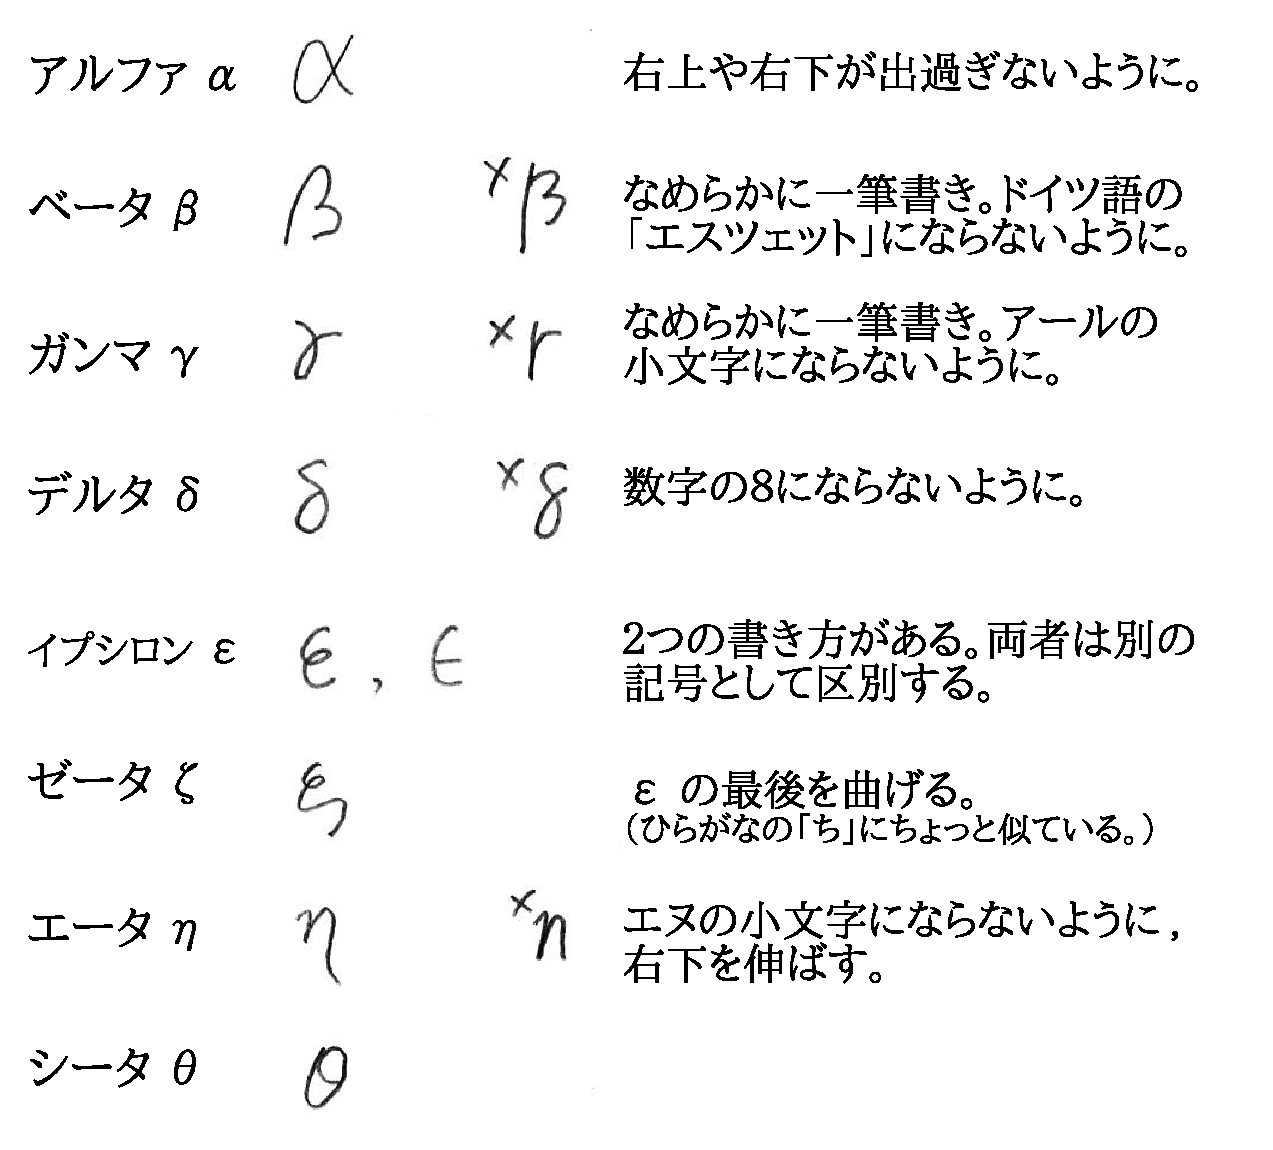
\includegraphics[width=7.5cm]{Greece1.eps}
    \caption{ギリシア文字の小文字($\alpha, \beta, \gamma, \delta, \epsilon, \zeta, \eta, \theta$)の書き方。$\times$がついているのは, よくある間違った書き方。\label{fig:Greece1}}
\end{figure}

\begin{figure}[H]
    \centering
    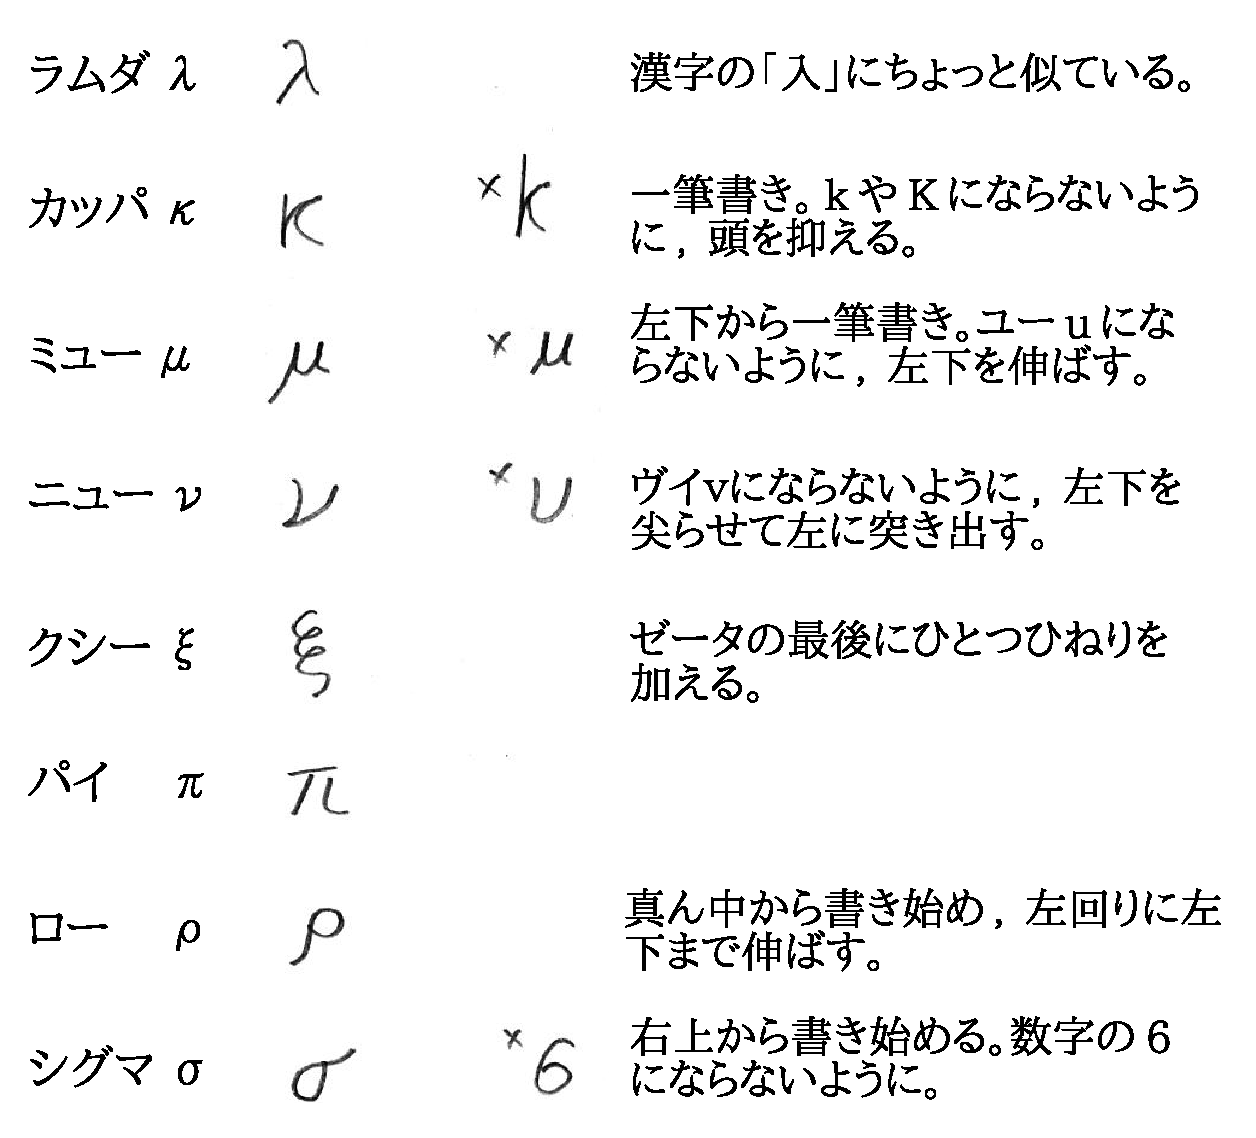
\includegraphics[width=7.5cm]{Greece2.eps}
    \caption{ギリシア文字の小文字($\lambda, \kappa, \mu, \nu, \xi, \pi, \rho, \sigma$)の書き方。$\times$がついているのは, よくある間違った書き方。\label{fig:Greece2}}
\end{figure}

\begin{figure}[H]
    \centering
    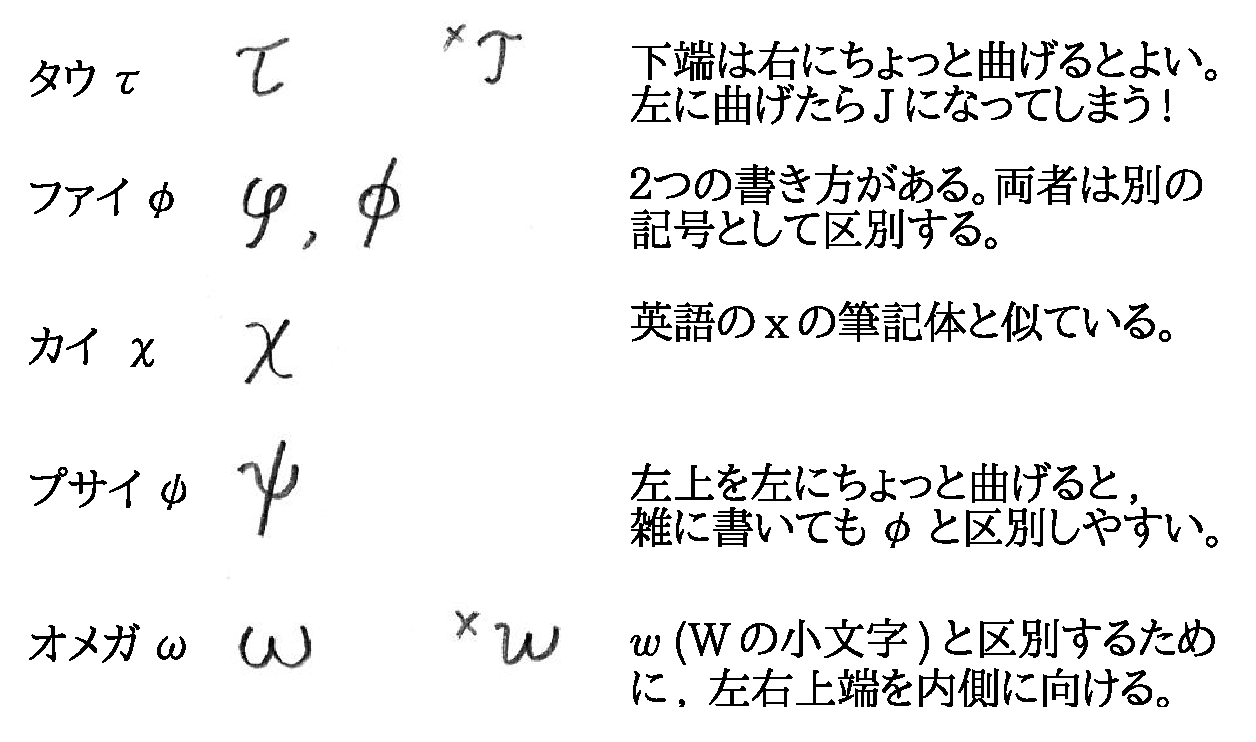
\includegraphics[width=7.5cm]{Greece3.eps}
    \caption{ギリシア文字の小文字($\tau, \phi, \chi, \psi, \omega$)の書き方。$\times$がついているのは, よくある間違った書き方。\label{fig:Greece3}}
\end{figure}

\begin{figure}[H]
    \centering
    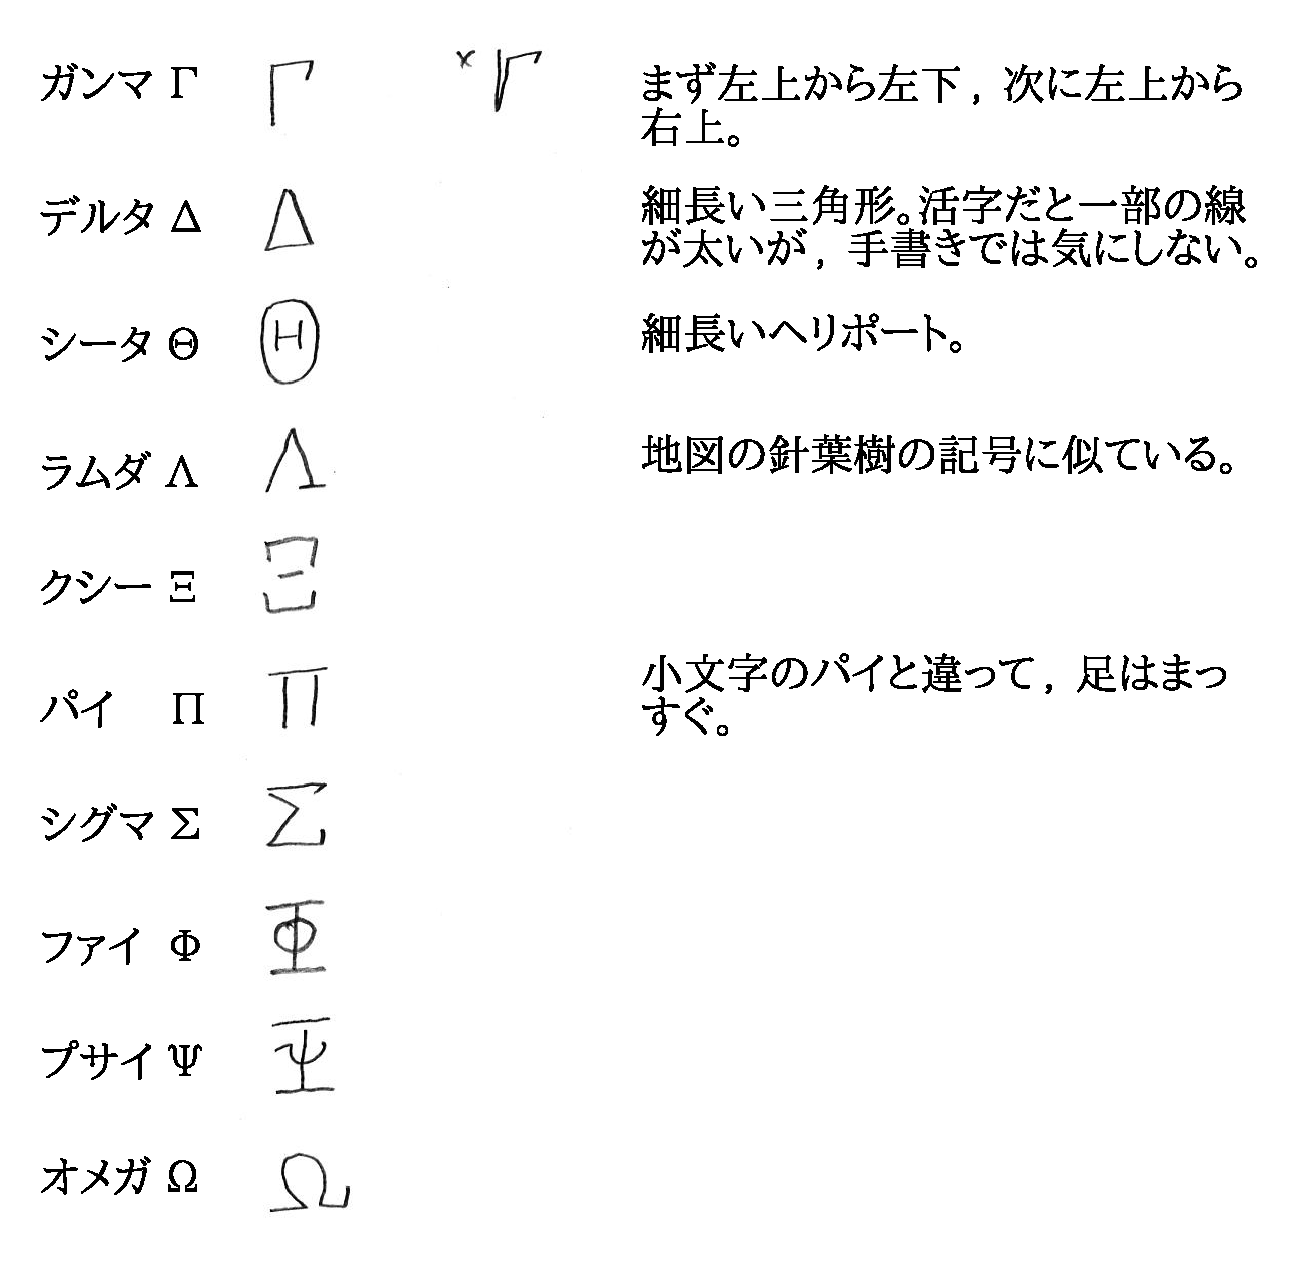
\includegraphics[width=7.5cm]{Greece4.eps}
    \caption{ギリシア文字の大文字($\Gamma, \Delta, \Theta, \Lambda, \Xi, \Pi, \Sigma, \Phi, \Psi, \Omega$)の書き方。$\times$がついているのは, よくある間違った書き方。\label{fig:Greece4}}
\end{figure}

\begin{freqmiss}{\small\textgt{以下の文字の書き分けができない: \\$\gamma$と$r$, $\delta$と$8$, 
$\eta$と$n$, $\kappa$と$k$, $\mu$と$u$, $\nu$と$v$, 
$\sigma$と$6$, $\chi$と$x$, $\omega$と$w$。}}\end{freqmiss}

\begin{faq}{\small\textgt{高校まで三角形を「$\triangle$」とかいていたのですが, 
デルタ「$\Delta$」と三角形「$\triangle$」は書き分けがあるのですか?}
... 手で書くときは, $\Delta$はちょっと細長く, しかも右に傾いた感じで書きます。
ちなみに$\triangle$は大学では「ラプラシアン」という概念を意味する記号でもあります。}\end{faq}

\begin{faq}{\small\textgt{$\Omega$って「オーム」じゃないんですか?}
... 中学校理科で習った電気抵抗の単位$\Omega$。これを「オーム」と呼ぶのは, 
「オームの法則」というのを発見したOhmさんという物理学者の名に由来します。
電流の単位をAと書いて「アンペア」と呼ぶのと同じようなものです
(アンペアはAmpereという物理学者の名に由来)。Ohmさんの頭文字だから, 
大文字のOにしたかったのでしょうけど, 数字の零と紛らわしいので, 
Oに対応するギリシア文字の$\Omega$を採用した, というわけです(多分)。}\end{faq}

\begin{faq}{\small\textgt{携帯電話の記号のところにギリシャ文字が入っているのですが, 
$\iota$や$o$とは何ですか?}
... それぞれイオタ, オミクロンといいます。数学ではあまり使いません。}\end{faq}

\begin{faq}{\small\textgt{$\xi$とか$\eta$とかって, これまで実際に見たこと
はありません。本当に使うのですか? }
... 大学で専門的な勉強をしていくと, いろんなところで出てきますよ。}\end{faq}
\mv


\section*{演習問題}

%\begin{exq}\label{q:unit_missing} 無限大$\infty$を数(実数)の
%ひとつとして認めてしまうと, どういう困ったことが生じるか, 四則演算の公理に
%基いて述べよ。\end{exq}

\begin{exq} 任意の自然数$x$について, $x$を10進法で表したとき, 
各桁の数(0以上9以下)を全部足したものが3で割り切れれば, $x$は3で
割り切れる。これを証明せよ。\end{exq}

\begin{exq}\label{q:div_by_zero} もし「0で割る」ことができるなら, どのような矛盾が生じるか?\end{exq}
%\noindent{\textbf{答}}\ref{q:div_by_zero} 
% もし$2\div 0$が可能ならば, その答を$x$とすれば, 
%$2\div 0=x$である。すると, 割り算の定義から, $2=0\times x=0$
%となり, $2=0$という, 変な等式が出てきてしまう。\\

\begin{exq}\label{q:base_zero} \eref{eq:taisuu00}のすぐ後に
「ただし$a\neq1$とする」という条件があった。もし$a=1$を考えると, 
どのような困ったことが起きるか?\end{exq}

%\答 $a=1$のとき, すなわち$\log_1 x$は, 「1を何乗したら$x$になるか?」である。
%ところが, 1は何乗しても1だから, $x=1$のときを除いて, $\log_1 x$は存在しないので, $\log_1 x$を考えるのはほとんど無意味である。\\

\begin{exq}\label{q:triangle_gravxenter} 三角形ABCの各頂点に, 
互いに等しい質量のおもりがくっついている。辺BCの中点をDとすると, 
この3つのおもりの重心は, 線分ADを2:1に内分する点にあることを, 
位置ベクトルを使って示せ。ヒント: A, B, Cの各位置ベクトルを${\bf a}$, 
${\bf b}$, ${\bf c}$とすると, 3つのおもりの重心の位置ベクトル${\bf r}$は, 
${\bf r}=({\bf a}+{\bf b}+{\bf c})/3$である(これは重心の定義)。
\end{exq}

%\begin{exq}\label{q:alg_def_speed} 速さの定義を述べよ, という問に, 
%C君は「進んだ距離(m)をかかった時間(秒)で割ったものを速さという」と答えた。
%これは定義として適切か?
%\end{exq}
%\noindent{\textbf{答}}\ref{q:alg_def_speed} 
%不適切。mや秒という単位まで指定するのは蛇足である。m以外の単位で距離を測り, 
%秒以外の単位で時間を測って割り算をしたものも「速さ」である。\\
\hv


\section*{問の解答}
{\small ここに解答が出ていない問題は, 解答が省略されている。各自, 自力で解こう。
また, 「略解」では最終的な答だけが述べられいるが, 君はきちんと導出過程も書くこと。\mv}

\noindent{\textbf{答}}\ref{q:badhabit_equality} 
ここでは「A君は学生である」の「は」を等号とみなしたのが間違い。
学生にはA君以外の人もいるし, A君は学生以外の属性(男性とか, 
茨城県出身とか, ...)も持つので, 「A君」と「学生」は同じではない。\mv

%\noindent{\textbf{答}}\ref{q:alg_num0} 自然数とは, 1を繰り返し足してできる数。整数とは, 自然数から自然数をひいてできる数。有理数とは, 整数を(0以外の)整数で割ってできる数。\mv

%\noindent{\textbf{答}}\ref{q:alg_def_pi} 「3.1415926, 以下, ずっと値が続く数」には, 3.1415926111...や, 3.1415926222...など, いろんな数があるので, この発言では円周率を特定できない。\mv

%\noindent{\textbf{答}}\ref{q:axiom_shisokuenzan} 略(がんばれ!)

%\noindent{\textbf{答}}\ref{q:th_zero} 略(本文の該当箇所をまとめればOK)

\noindent{\textbf{答}}\ref{q:bad_notation0} (1) $a$が分母なのか分子なのか
わからない。(2) $3\times(-4)$と書くべき。(3) 二重括弧は外側を\{\}に。また, 末尾の$x$が
分母なのか分子なのかわからない。

%\noindent{\textbf{答}}\ref{q:alg_order2}
%\begin{enumerate}
%\item \eref{eq:axiom_order2}で, $c=-a$とすれば, $a-a<b-a$。
%この左辺は, \eref{eq:axiom_num_sum_inv}より0。従って$0<b-a$。
%\item $a<b$のとき, 前小問より$0<b-a$。\eref{eq:axiom_order3}で
%$a$を$c$に, $b$を$b-a$に置き換えれば, $0<c(b-a)$。
%この右辺は, \eref{eq:axiom_num_distr}で$a$を$c$に, $b$は$b$のままに, 
%$c$を$-a$に置き換えれば, $cb-ca$となる(以下, このような置き換えに
%ついての記述は省略する)。従って, $0<cb-ca$。両辺に
%$ca$を足せば, \eref{eq:axiom_order2}より$ca<cb$。\eref{eq:axiom_num_mult_exch}
%を両辺に適用して, $ac<bc$。
%\item $c<0$の両辺に$-c$を足すと(\eref{eq:axiom_order2}より)$0<-c$となる。
%前小問の$c$を$-c$に置き換えれば, $a(-c)<b(-c)$。従って, $-ac<-bc$。この
%両辺に$ac+bc$を足せば, $-ac+(ac+bc)<-bc+(ac+bc)$。\eref{eq:axiom_num_sum_assoc}を
%左辺に使えば, 左辺=$(-ac+ac)+bc=bc$。\eref{eq:axiom_num_sum_exch}を右辺に使い, 
%続けて\eref{eq:axiom_num_sum_assoc}を使えば, 右辺=$(ac+bc)-bc=ac+(bc-bc)=ac$。
%従って, $bc<ac$。
%\end{enumerate}

%\noindent{\textbf{答}}\ref{q:alg_ineq3} 略。
%$|a^2|=|a|^2=a^2,\, |a||b|=|ab|$等に注意。
%\begin{enumerate}
%\item 略(左辺を展開)
%\item $0\leq a+b$のとき, \eref{eq:alg_abs1}の$a$を$a+b$で置き換えて考えれば, $|a+b|=a+b$である。
%従って, $|a+b|^2=(a+b)^2=a^2+2ab+b^2$。\\
%$a+b<0$のとき, \eref{eq:alg_abs2}の$a$を$a+b$で置き換えて考えれば, $|a+b|=-(a+b)$である。
%従って, $|a+b|^2=\{-(a+b)%\}^2=(a+b)^2=a^2+2ab+b^2$。
%\item (1)$-$(2)より明らか。
%\item $|ab|$は$ab$と等しいか($ab \ge0$のとき), $ab$より大きい($ab<0$のとき)。
%従って, $ab \le |ab|$。よって$0 \le |ab|-ab$。
%\item (3)(4)より, 明らか。
%\item 絶対値か, 絶対値の足し算だから, 0以上なのは自明。
%\item (6)と命題8より, (5)の両辺の平方根をとっても不等号の向きはかわらない。
%\end{enumerate}
\mv

\noindent{\textbf{答}}\ref{q:alg_pow0} (1) 32 (2) $1/2^2= 1/4$ (3) $10^{-2} = 1/100$
(4) $9^{1/2} = \sqrt{9} = 3$ (5) 1 (6) $10^4$\mv

\noindent{\textbf{答}}\ref{q:alg_pow1} (1) $\,\,\,3^{-1/2}\,\,\,\,\,\,\,\,$ (2) $\,\,\,5^{1/3}$
\mv

\begin{comment}
\noindent{\textbf{答}}\ref{q:sqrt_ab} 
\begin{enumerate}
\item 
$(\sqrt{a}\,\sqrt{b})^2=\sqrt{a}\,\sqrt{b}\,\sqrt{a}\,\sqrt{b}
=\sqrt{a}\,\sqrt{a}\,\sqrt{b}\,\sqrt{b}=(\sqrt{a})^2\,(\sqrt{b})^2=ab$。
また, $\sqrt{a}\geq0$, $\sqrt{b}\geq0$は自明だから, $\sqrt{a}\,\sqrt{b}\geq0$。
すなわち$\sqrt{a}\,\sqrt{b}$は$ab$の0以上の平方根。すなわち, 
$\sqrt{a}\,\sqrt{b}=\sqrt{ab}$。\qed
%ちなみに, この考え方を発展させれば, 任意の実数$\alpha$について, 
%$(ab)^\alpha=a^\alpha b^\alpha$が証明できる。
\item $\sqrt{10}=\sqrt{2\cdot5}=\sqrt{2}\sqrt{5}=1.414\cdots\times2.236\cdots=3.162\cdots\fallingdotseq3.16$。
これは, $\pi=3.1415\cdots$より大きい。注: $\sqrt{10}$が$\pi$に非常に近い数であるということは, 
豆知識として知っておいて損はない。
\end{enumerate}
\end{comment}

\noindent{\textbf{答}}\ref{q:alg_dentaku2} (?は秘密!) (1) 11.313?? (2) 2.704?? (3) 1.709??\mv

%\noindent{\textbf{答}}\ref{q:Napier_value_memorize} 略。(がんばれ!)\mv

\noindent{\textbf{答}}\ref{q:alg_dentaku_exp} 略解として小数第3位までで打ち切った値を示す。
レポートでは小数5位まで書くこと。\\(1) 7.389 (2) 0.223\mv

\noindent{\textbf{答}}\ref{q:exp_logvalue0} (1) $2$ (2) $4$ (3) $2$ (4) $3$ (5) $-2$ (6) $0$\mv

%\noindent{\textbf{答}}\ref{q:whatis_log} 略。\mv

\noindent{\textbf{答}}\ref{q:alg_dentaku_ln} 
略解として小数第3位までで打ち切った値を示す。
レポートでは小数5位まで書くこと。(1) 0.301 (2) $-2.221$ (3) 0.693 (4) 2.302\mv

%\noindent{\textbf{答}}\ref{q:vect_write} 略。(がんばれ!)\mv

\noindent{\textbf{答}}\ref{q:vect_add_fig} 略。図の上に作図してみよ。
ベクトルはどこに置くかを問題としないことに注意!
\mv

% 点A(4, 5)と点B(3, 6)について,
\noindent{\textbf{答}}\ref{q:vect_pos2D}  点A, Bの位置ベクトルをそれぞれ${\bf a}$, ${\bf b}$とすると
\begin{eqnarray*}\text(1)\quad\frac{2{\bf a}+{\bf b}}{3}=\Bigl(\frac{11}{3}, \frac{16}{3}\Bigr)\quad\quad
                 \text(2)\quad\frac{{\bf a}+2{\bf b}}{3}=\Bigl(\frac{10}{3}, \frac{17}{3}\Bigr)\end{eqnarray*}

\noindent{\textbf{答}}\ref{q:guard_digit_order} 
(1) 5, 3の2桁。 (2) 1, 2, 3, 0, 5の5桁。 (3) 5, 3は確実に有効数字だが, 
そのあとの2つの0は有効数字かどうかわからない。 (4) 2, 3, 0の3桁。\mv

\noindent{\textbf{答}}\ref{q:guard_digit_prac2} (1) 11.9 (2) 123.5 (3) 87\mv

\noindent{\textbf{答}}\ref{q:guard_digit_prac4} (1) 14 (2) 2.8 (3) 7.7\mv

\noindent{\textbf{答}}\ref{q:guard_digit_8} (1) 12.8 cm (2) 13 cm 
(3) 略(君の考えを正直に述べよ)\mv

\noindent{\textbf{答}}\ref{q:guard_digit_9} 
(1) 13.1から13.3までなので, 0.1の桁が不確定と見て, 13.2。 (2) 13.0から13.4までなので, 
これも0.1の桁が不確定と見て, 13.2。 (3) 12.6から13.8までなので, 1の桁が不確定とみて, 
13。

%\noindent{\textbf{答}}\ref{q:logic_Greece} 略。(がんばれ!)


%\begin{faq}{\small\textgt{演習問題の答が欲しいです} ... 考えることを楽しんで欲しいので, あえて載せていません。どうしても知りたければ質問においで。一緒に考えよう!}\end{faq}

%\begin{faq}{\small\textgt{勉強すれば本当に数学が好きになりますか? リメディアル教材の内容を出来るようになる自信がありません} ... 「はじめに」に載っている勉強法を守って丁寧にやれば大丈夫。そうすると, だんだん楽しくなって, 数学が好きになってきます。やみくもに焦ってストイックに頑張るだけでは, すぐに心折れちゃって, 数学が嫌いになっちゃうよ。}\end{faq}

%\begin{faq}\small{\textgt{大学で高校数学の復習なんて, ゆるくないですか?}... ゆるくないです。高校数学の復習は, 全ての大学生に必要です。高校数学は, 大学入試の問題演習が中心ですので, 「問題は解けるけど, 基礎を理解していない」という人が多いのです。そんな状態のままで大学数学を詰め込まれ, 消化不良を起こして脱落する大学生がたくさんいます。}\end{faq}


